\documentclass{article} % For LaTeX2e
\usepackage{iclr2027_conference,times}
\usepackage{booktabs}
\usepackage{caption}
\usepackage{multirow}
\usepackage{listings}
\usepackage[most]{tcolorbox}
\usepackage[utf8]{inputenc} % allow utf-8 input
\usepackage[T1]{fontenc}    % use 8-bit T1 fonts
\usepackage{hyperref}       % hyperlinks
\usepackage{url}            % simple URL typesetting
\usepackage{booktabs}       % professional-quality tables
\usepackage{amsfonts}       % blackboard math symbols
\usepackage{nicefrac}       % compact symbols for 1/2, etc.
\usepackage{microtype}      % microtypography
\usepackage{xcolor}         % colors

\usepackage{pifont}
\usepackage{multirow}
\definecolor{darkgreen}{rgb}{0, 0.5, 0} % 暗绿色
\definecolor{darkred}{rgb}{0.8, 0, 0}  % 暗红色
\newcommand{\greencheck}{\textcolor{darkgreen}{\ding{51}}}
\newcommand{\redcross}{\textcolor{darkred}{\ding{55}}}

\input{qiushi_custom}

% Optional math commands from https://github.com/goodfeli/dlbook_notation.
%%%%% NEW MATH DEFINITIONS %%%%%

\usepackage{amsmath,amsfonts,bm}

% Mark sections of captions for referring to divisions of figures
\newcommand{\figleft}{{\em (Left)}}
\newcommand{\figcenter}{{\em (Center)}}
\newcommand{\figright}{{\em (Right)}}
\newcommand{\figtop}{{\em (Top)}}
\newcommand{\figbottom}{{\em (Bottom)}}
\newcommand{\captiona}{{\em (a)}}
\newcommand{\captionb}{{\em (b)}}
\newcommand{\captionc}{{\em (c)}}
\newcommand{\captiond}{{\em (d)}}

% Highlight a newly defined term
\newcommand{\newterm}[1]{{\bf #1}}


% Figure reference, lower-case.
\def\figref#1{figure~\ref{#1}}
% Figure reference, capital. For start of sentence
\def\Figref#1{Figure~\ref{#1}}
\def\twofigref#1#2{figures \ref{#1} and \ref{#2}}
\def\quadfigref#1#2#3#4{figures \ref{#1}, \ref{#2}, \ref{#3} and \ref{#4}}
% Section reference, lower-case.
\def\secref#1{section~\ref{#1}}
% Section reference, capital.
\def\Secref#1{Section~\ref{#1}}
% Reference to two sections.
\def\twosecrefs#1#2{sections \ref{#1} and \ref{#2}}
% Reference to three sections.
\def\secrefs#1#2#3{sections \ref{#1}, \ref{#2} and \ref{#3}}
% Reference to an equation, lower-case.
\def\eqref#1{equation~\ref{#1}}
% Reference to an equation, upper case
\def\Eqref#1{Equation~\ref{#1}}
% A raw reference to an equation---avoid using if possible
\def\plaineqref#1{\ref{#1}}
% Reference to a chapter, lower-case.
\def\chapref#1{chapter~\ref{#1}}
% Reference to an equation, upper case.
\def\Chapref#1{Chapter~\ref{#1}}
% Reference to a range of chapters
\def\rangechapref#1#2{chapters\ref{#1}--\ref{#2}}
% Reference to an algorithm, lower-case.
\def\algref#1{algorithm~\ref{#1}}
% Reference to an algorithm, upper case.
\def\Algref#1{Algorithm~\ref{#1}}
\def\twoalgref#1#2{algorithms \ref{#1} and \ref{#2}}
\def\Twoalgref#1#2{Algorithms \ref{#1} and \ref{#2}}
% Reference to a part, lower case
\def\partref#1{part~\ref{#1}}
% Reference to a part, upper case
\def\Partref#1{Part~\ref{#1}}
\def\twopartref#1#2{parts \ref{#1} and \ref{#2}}

\def\ceil#1{\lceil #1 \rceil}
\def\floor#1{\lfloor #1 \rfloor}
\def\1{\bm{1}}
\newcommand{\train}{\mathcal{D}}
\newcommand{\valid}{\mathcal{D_{\mathrm{valid}}}}
\newcommand{\test}{\mathcal{D_{\mathrm{test}}}}

\def\eps{{\epsilon}}


% Random variables
\def\reta{{\textnormal{$\eta$}}}
\def\ra{{\textnormal{a}}}
\def\rb{{\textnormal{b}}}
\def\rc{{\textnormal{c}}}
\def\rd{{\textnormal{d}}}
\def\re{{\textnormal{e}}}
\def\rf{{\textnormal{f}}}
\def\rg{{\textnormal{g}}}
\def\rh{{\textnormal{h}}}
\def\ri{{\textnormal{i}}}
\def\rj{{\textnormal{j}}}
\def\rk{{\textnormal{k}}}
\def\rl{{\textnormal{l}}}
% rm is already a command, just don't name any random variables m
\def\rn{{\textnormal{n}}}
\def\ro{{\textnormal{o}}}
\def\rp{{\textnormal{p}}}
\def\rq{{\textnormal{q}}}
\def\rr{{\textnormal{r}}}
\def\rs{{\textnormal{s}}}
\def\rt{{\textnormal{t}}}
\def\ru{{\textnormal{u}}}
\def\rv{{\textnormal{v}}}
\def\rw{{\textnormal{w}}}
\def\rx{{\textnormal{x}}}
\def\ry{{\textnormal{y}}}
\def\rz{{\textnormal{z}}}

% Random vectors
\def\rvepsilon{{\mathbf{\epsilon}}}
\def\rvtheta{{\mathbf{\theta}}}
\def\rva{{\mathbf{a}}}
\def\rvb{{\mathbf{b}}}
\def\rvc{{\mathbf{c}}}
\def\rvd{{\mathbf{d}}}
\def\rve{{\mathbf{e}}}
\def\rvf{{\mathbf{f}}}
\def\rvg{{\mathbf{g}}}
\def\rvh{{\mathbf{h}}}
\def\rvu{{\mathbf{i}}}
\def\rvj{{\mathbf{j}}}
\def\rvk{{\mathbf{k}}}
\def\rvl{{\mathbf{l}}}
\def\rvm{{\mathbf{m}}}
\def\rvn{{\mathbf{n}}}
\def\rvo{{\mathbf{o}}}
\def\rvp{{\mathbf{p}}}
\def\rvq{{\mathbf{q}}}
\def\rvr{{\mathbf{r}}}
\def\rvs{{\mathbf{s}}}
\def\rvt{{\mathbf{t}}}
\def\rvu{{\mathbf{u}}}
\def\rvv{{\mathbf{v}}}
\def\rvw{{\mathbf{w}}}
\def\rvx{{\mathbf{x}}}
\def\rvy{{\mathbf{y}}}
\def\rvz{{\mathbf{z}}}

% Elements of random vectors
\def\erva{{\textnormal{a}}}
\def\ervb{{\textnormal{b}}}
\def\ervc{{\textnormal{c}}}
\def\ervd{{\textnormal{d}}}
\def\erve{{\textnormal{e}}}
\def\ervf{{\textnormal{f}}}
\def\ervg{{\textnormal{g}}}
\def\ervh{{\textnormal{h}}}
\def\ervi{{\textnormal{i}}}
\def\ervj{{\textnormal{j}}}
\def\ervk{{\textnormal{k}}}
\def\ervl{{\textnormal{l}}}
\def\ervm{{\textnormal{m}}}
\def\ervn{{\textnormal{n}}}
\def\ervo{{\textnormal{o}}}
\def\ervp{{\textnormal{p}}}
\def\ervq{{\textnormal{q}}}
\def\ervr{{\textnormal{r}}}
\def\ervs{{\textnormal{s}}}
\def\ervt{{\textnormal{t}}}
\def\ervu{{\textnormal{u}}}
\def\ervv{{\textnormal{v}}}
\def\ervw{{\textnormal{w}}}
\def\ervx{{\textnormal{x}}}
\def\ervy{{\textnormal{y}}}
\def\ervz{{\textnormal{z}}}

% Random matrices
\def\rmA{{\mathbf{A}}}
\def\rmB{{\mathbf{B}}}
\def\rmC{{\mathbf{C}}}
\def\rmD{{\mathbf{D}}}
\def\rmE{{\mathbf{E}}}
\def\rmF{{\mathbf{F}}}
\def\rmG{{\mathbf{G}}}
\def\rmH{{\mathbf{H}}}
\def\rmI{{\mathbf{I}}}
\def\rmJ{{\mathbf{J}}}
\def\rmK{{\mathbf{K}}}
\def\rmL{{\mathbf{L}}}
\def\rmM{{\mathbf{M}}}
\def\rmN{{\mathbf{N}}}
\def\rmO{{\mathbf{O}}}
\def\rmP{{\mathbf{P}}}
\def\rmQ{{\mathbf{Q}}}
\def\rmR{{\mathbf{R}}}
\def\rmS{{\mathbf{S}}}
\def\rmT{{\mathbf{T}}}
\def\rmU{{\mathbf{U}}}
\def\rmV{{\mathbf{V}}}
\def\rmW{{\mathbf{W}}}
\def\rmX{{\mathbf{X}}}
\def\rmY{{\mathbf{Y}}}
\def\rmZ{{\mathbf{Z}}}

% Elements of random matrices
\def\ermA{{\textnormal{A}}}
\def\ermB{{\textnormal{B}}}
\def\ermC{{\textnormal{C}}}
\def\ermD{{\textnormal{D}}}
\def\ermE{{\textnormal{E}}}
\def\ermF{{\textnormal{F}}}
\def\ermG{{\textnormal{G}}}
\def\ermH{{\textnormal{H}}}
\def\ermI{{\textnormal{I}}}
\def\ermJ{{\textnormal{J}}}
\def\ermK{{\textnormal{K}}}
\def\ermL{{\textnormal{L}}}
\def\ermM{{\textnormal{M}}}
\def\ermN{{\textnormal{N}}}
\def\ermO{{\textnormal{O}}}
\def\ermP{{\textnormal{P}}}
\def\ermQ{{\textnormal{Q}}}
\def\ermR{{\textnormal{R}}}
\def\ermS{{\textnormal{S}}}
\def\ermT{{\textnormal{T}}}
\def\ermU{{\textnormal{U}}}
\def\ermV{{\textnormal{V}}}
\def\ermW{{\textnormal{W}}}
\def\ermX{{\textnormal{X}}}
\def\ermY{{\textnormal{Y}}}
\def\ermZ{{\textnormal{Z}}}

% Vectors
\def\vzero{{\bm{0}}}
\def\vone{{\bm{1}}}
\def\vmu{{\bm{\mu}}}
\def\vtheta{{\bm{\theta}}}
\def\va{{\bm{a}}}
\def\vb{{\bm{b}}}
\def\vc{{\bm{c}}}
\def\vd{{\bm{d}}}
\def\ve{{\bm{e}}}
\def\vf{{\bm{f}}}
\def\vg{{\bm{g}}}
\def\vh{{\bm{h}}}
\def\vi{{\bm{i}}}
\def\vj{{\bm{j}}}
\def\vk{{\bm{k}}}
\def\vl{{\bm{l}}}
\def\vm{{\bm{m}}}
\def\vn{{\bm{n}}}
\def\vo{{\bm{o}}}
\def\vp{{\bm{p}}}
\def\vq{{\bm{q}}}
\def\vr{{\bm{r}}}
\def\vs{{\bm{s}}}
\def\vt{{\bm{t}}}
\def\vu{{\bm{u}}}
\def\vv{{\bm{v}}}
\def\vw{{\bm{w}}}
\def\vx{{\bm{x}}}
\def\vy{{\bm{y}}}
\def\vz{{\bm{z}}}

% Elements of vectors
\def\evalpha{{\alpha}}
\def\evbeta{{\beta}}
\def\evepsilon{{\epsilon}}
\def\evlambda{{\lambda}}
\def\evomega{{\omega}}
\def\evmu{{\mu}}
\def\evpsi{{\psi}}
\def\evsigma{{\sigma}}
\def\evtheta{{\theta}}
\def\eva{{a}}
\def\evb{{b}}
\def\evc{{c}}
\def\evd{{d}}
\def\eve{{e}}
\def\evf{{f}}
\def\evg{{g}}
\def\evh{{h}}
\def\evi{{i}}
\def\evj{{j}}
\def\evk{{k}}
\def\evl{{l}}
\def\evm{{m}}
\def\evn{{n}}
\def\evo{{o}}
\def\evp{{p}}
\def\evq{{q}}
\def\evr{{r}}
\def\evs{{s}}
\def\evt{{t}}
\def\evu{{u}}
\def\evv{{v}}
\def\evw{{w}}
\def\evx{{x}}
\def\evy{{y}}
\def\evz{{z}}

% Matrix
\def\mA{{\bm{A}}}
\def\mB{{\bm{B}}}
\def\mC{{\bm{C}}}
\def\mD{{\bm{D}}}
\def\mE{{\bm{E}}}
\def\mF{{\bm{F}}}
\def\mG{{\bm{G}}}
\def\mH{{\bm{H}}}
\def\mI{{\bm{I}}}
\def\mJ{{\bm{J}}}
\def\mK{{\bm{K}}}
\def\mL{{\bm{L}}}
\def\mM{{\bm{M}}}
\def\mN{{\bm{N}}}
\def\mO{{\bm{O}}}
\def\mP{{\bm{P}}}
\def\mQ{{\bm{Q}}}
\def\mR{{\bm{R}}}
\def\mS{{\bm{S}}}
\def\mT{{\bm{T}}}
\def\mU{{\bm{U}}}
\def\mV{{\bm{V}}}
\def\mW{{\bm{W}}}
\def\mX{{\bm{X}}}
\def\mY{{\bm{Y}}}
\def\mZ{{\bm{Z}}}
\def\mBeta{{\bm{\beta}}}
\def\mPhi{{\bm{\Phi}}}
\def\mLambda{{\bm{\Lambda}}}
\def\mSigma{{\bm{\Sigma}}}

% Tensor
\DeclareMathAlphabet{\mathsfit}{\encodingdefault}{\sfdefault}{m}{sl}
\SetMathAlphabet{\mathsfit}{bold}{\encodingdefault}{\sfdefault}{bx}{n}
\newcommand{\tens}[1]{\bm{\mathsfit{#1}}}
\def\tA{{\tens{A}}}
\def\tB{{\tens{B}}}
\def\tC{{\tens{C}}}
\def\tD{{\tens{D}}}
\def\tE{{\tens{E}}}
\def\tF{{\tens{F}}}
\def\tG{{\tens{G}}}
\def\tH{{\tens{H}}}
\def\tI{{\tens{I}}}
\def\tJ{{\tens{J}}}
\def\tK{{\tens{K}}}
\def\tL{{\tens{L}}}
\def\tM{{\tens{M}}}
\def\tN{{\tens{N}}}
\def\tO{{\tens{O}}}
\def\tP{{\tens{P}}}
\def\tQ{{\tens{Q}}}
\def\tR{{\tens{R}}}
\def\tS{{\tens{S}}}
\def\tT{{\tens{T}}}
\def\tU{{\tens{U}}}
\def\tV{{\tens{V}}}
\def\tW{{\tens{W}}}
\def\tX{{\tens{X}}}
\def\tY{{\tens{Y}}}
\def\tZ{{\tens{Z}}}


% Graph
\def\gA{{\mathcal{A}}}
\def\gB{{\mathcal{B}}}
\def\gC{{\mathcal{C}}}
\def\gD{{\mathcal{D}}}
\def\gE{{\mathcal{E}}}
\def\gF{{\mathcal{F}}}
\def\gG{{\mathcal{G}}}
\def\gH{{\mathcal{H}}}
\def\gI{{\mathcal{I}}}
\def\gJ{{\mathcal{J}}}
\def\gK{{\mathcal{K}}}
\def\gL{{\mathcal{L}}}
\def\gM{{\mathcal{M}}}
\def\gN{{\mathcal{N}}}
\def\gO{{\mathcal{O}}}
\def\gP{{\mathcal{P}}}
\def\gQ{{\mathcal{Q}}}
\def\gR{{\mathcal{R}}}
\def\gS{{\mathcal{S}}}
\def\gT{{\mathcal{T}}}
\def\gU{{\mathcal{U}}}
\def\gV{{\mathcal{V}}}
\def\gW{{\mathcal{W}}}
\def\gX{{\mathcal{X}}}
\def\gY{{\mathcal{Y}}}
\def\gZ{{\mathcal{Z}}}

% Sets
\def\sA{{\mathbb{A}}}
\def\sB{{\mathbb{B}}}
\def\sC{{\mathbb{C}}}
\def\sD{{\mathbb{D}}}
% Don't use a set called E, because this would be the same as our symbol
% for expectation.
\def\sF{{\mathbb{F}}}
\def\sG{{\mathbb{G}}}
\def\sH{{\mathbb{H}}}
\def\sI{{\mathbb{I}}}
\def\sJ{{\mathbb{J}}}
\def\sK{{\mathbb{K}}}
\def\sL{{\mathbb{L}}}
\def\sM{{\mathbb{M}}}
\def\sN{{\mathbb{N}}}
\def\sO{{\mathbb{O}}}
\def\sP{{\mathbb{P}}}
\def\sQ{{\mathbb{Q}}}
\def\sR{{\mathbb{R}}}
\def\sS{{\mathbb{S}}}
\def\sT{{\mathbb{T}}}
\def\sU{{\mathbb{U}}}
\def\sV{{\mathbb{V}}}
\def\sW{{\mathbb{W}}}
\def\sX{{\mathbb{X}}}
\def\sY{{\mathbb{Y}}}
\def\sZ{{\mathbb{Z}}}

% Entries of a matrix
\def\emLambda{{\Lambda}}
\def\emA{{A}}
\def\emB{{B}}
\def\emC{{C}}
\def\emD{{D}}
\def\emE{{E}}
\def\emF{{F}}
\def\emG{{G}}
\def\emH{{H}}
\def\emI{{I}}
\def\emJ{{J}}
\def\emK{{K}}
\def\emL{{L}}
\def\emM{{M}}
\def\emN{{N}}
\def\emO{{O}}
\def\emP{{P}}
\def\emQ{{Q}}
\def\emR{{R}}
\def\emS{{S}}
\def\emT{{T}}
\def\emU{{U}}
\def\emV{{V}}
\def\emW{{W}}
\def\emX{{X}}
\def\emY{{Y}}
\def\emZ{{Z}}
\def\emSigma{{\Sigma}}

% entries of a tensor
% Same font as tensor, without \bm wrapper
\newcommand{\etens}[1]{\mathsfit{#1}}
\def\etLambda{{\etens{\Lambda}}}
\def\etA{{\etens{A}}}
\def\etB{{\etens{B}}}
\def\etC{{\etens{C}}}
\def\etD{{\etens{D}}}
\def\etE{{\etens{E}}}
\def\etF{{\etens{F}}}
\def\etG{{\etens{G}}}
\def\etH{{\etens{H}}}
\def\etI{{\etens{I}}}
\def\etJ{{\etens{J}}}
\def\etK{{\etens{K}}}
\def\etL{{\etens{L}}}
\def\etM{{\etens{M}}}
\def\etN{{\etens{N}}}
\def\etO{{\etens{O}}}
\def\etP{{\etens{P}}}
\def\etQ{{\etens{Q}}}
\def\etR{{\etens{R}}}
\def\etS{{\etens{S}}}
\def\etT{{\etens{T}}}
\def\etU{{\etens{U}}}
\def\etV{{\etens{V}}}
\def\etW{{\etens{W}}}
\def\etX{{\etens{X}}}
\def\etY{{\etens{Y}}}
\def\etZ{{\etens{Z}}}

% The true underlying data generating distribution
\newcommand{\pdata}{p_{\rm{data}}}
% The empirical distribution defined by the training set
\newcommand{\ptrain}{\hat{p}_{\rm{data}}}
\newcommand{\Ptrain}{\hat{P}_{\rm{data}}}
% The model distribution
\newcommand{\pmodel}{p_{\rm{model}}}
\newcommand{\Pmodel}{P_{\rm{model}}}
\newcommand{\ptildemodel}{\tilde{p}_{\rm{model}}}
% Stochastic autoencoder distributions
\newcommand{\pencode}{p_{\rm{encoder}}}
\newcommand{\pdecode}{p_{\rm{decoder}}}
\newcommand{\precons}{p_{\rm{reconstruct}}}

\newcommand{\laplace}{\mathrm{Laplace}} % Laplace distribution

\newcommand{\E}{\mathbb{E}}
\newcommand{\Ls}{\mathcal{L}}
\newcommand{\R}{\mathbb{R}}
\newcommand{\emp}{\tilde{p}}
\newcommand{\lr}{\alpha}
\newcommand{\reg}{\lambda}
\newcommand{\rect}{\mathrm{rectifier}}
\newcommand{\softmax}{\mathrm{softmax}}
\newcommand{\sigmoid}{\sigma}
\newcommand{\softplus}{\zeta}
\newcommand{\KL}{D_{\mathrm{KL}}}
\newcommand{\Var}{\mathrm{Var}}
\newcommand{\standarderror}{\mathrm{SE}}
\newcommand{\Cov}{\mathrm{Cov}}
% Wolfram Mathworld says $L^2$ is for function spaces and $\ell^2$ is for vectors
% But then they seem to use $L^2$ for vectors throughout the site, and so does
% wikipedia.
\newcommand{\normlzero}{L^0}
\newcommand{\normlone}{L^1}
\newcommand{\normltwo}{L^2}
\newcommand{\normlp}{L^p}
\newcommand{\normmax}{L^\infty}

\newcommand{\parents}{Pa} % See usage in notation.tex. Chosen to match Daphne's book.

\DeclareMathOperator*{\argmax}{arg\,max}
\DeclareMathOperator*{\argmin}{arg\,min}

\DeclareMathOperator{\sign}{sign}
\DeclareMathOperator{\Tr}{Tr}
\let\ab\allowbreak


% Shared macros used across chapters. Add new commands here, not in chapter files.
% Shared macros and notation. Only one person should add a new command at a time
% to avoid git conflicts. Do not \newcommand the same name in a chapter file.

% Example:
% \newcommand{\model}{\textsc{ModelName}}
% \newcommand{\dataset}{\textsc{DatasetName}}

% Put your custom macros here
\usepackage{fvextra}
\usepackage[most]{tcolorbox}
\newcommand{\promptfile}[3][]{%
  \begin{tcolorbox}[
    title={#2},
    breakable,
    enhanced,
    colback=gray!4,
    colframe=gray!65!black,
    colbacktitle=gray!65!black,
    fonttitle=\bfseries\small,
    boxrule=0.6pt,
    arc=2pt,
    left=4pt, right=4pt, top=2pt, bottom=2pt,
    #1]
  \VerbatimInput[
    fontsize=\scriptsize,
    breaklines=true,
    breakanywhere=true,
    breakindent=0pt,
    breaksymbolleft={\textcolor{gray}{\tiny$\hookrightarrow$}},
  ]{#3}
  \end{tcolorbox}%
}

\usepackage{hyperref}
\usepackage{url}
\usepackage{graphicx}
\usepackage{float}
% =============================================================================
% Collaboration notes
% -----------------------------------------------------------------------------
% Compile from the project root:
%   pdflatex main && bibtex main && pdflatex main && pdflatex main
%
% Each person edits only their file under chapters/. Do not put \section
% content in this file. To reduce git conflicts:
%   - Add citations to iclr2027_conference.bib (or your own .bib keys)
%   - Add \newcommand / notation to macros.tex
%   - Put figures in figures/ and reference them as figures/xxx.pdf
%   - Prefix labels with the chapter id, e.g. \label{sec:intro}, \label{fig:method-arch}
%
% Owner of this file (title / authors / abstract / package list): first author
% =============================================================================

% \title{OpenMobile-2: Advancing Mobile GUI Agents with Diverse Environments, High-Quality Data, and Hybrid GUI-MCP Interaction}

\title{OpenMobile-2: Building Versatile Mobile Agents with Scalable Environments and App-Native Tools}


% Authors must not appear in the submitted version. They should be hidden
% as long as the \iclrfinalcopy macro remains commented out below.
\author{Author One \thanks{Equal contribution.} \\
Affiliation \\
\texttt{email@example.com} \\
\And
Author Two \\
Affiliation \\
\texttt{email@example.com} \\
\AND
Author Three \\
Affiliation \\
\texttt{email@example.com}
}

\newcommand{\fix}{\marginpar{FIX}}
\newcommand{\new}{\marginpar{NEW}}
\newsavebox{\fighybridbox}

%\iclrfinalcopy % Uncomment for camera-ready version, but NOT for submission.
\begin{document}

\maketitle

\begin{abstract}
% Owner: first author (everyone can suggest, one person merges)
We introduce OpenMobile-2, a near-frontier mobile agent with fully open training environments and recipes. We make three key advances: (1) \textit{Diverse environments with simulated commercial apps}: We build \textsc{MobileGym++}, featuring 35 realistic, functionally rich commercial-style apps with cross-app workflows, while preserving full controllability for reset and verification. Together with newly configured apps in Android emulators, this yields a diverse playground spanning over 110 apps. (2) \textit{Open training data at scale}: Building on this foundation, we curate 12K mobile interaction trajectories for supervised fine-tuning and the largest open collection of verifiable RL training data for mobile agents, comprising over 2K executable tasks with automatic rewards. (3) \textit{Hybrid GUI and app-native tool use}: We explore an experimental mobile-use setting where apps expose selected functionalities as app-native tools alongside their GUIs, allowing agents to interleave GUI actions and tool calls within a task. We implement this setting in \textsc{MobileGym++} with over 300 carefully scoped tools across 50 apps. Additionally, we introduce \textsc{MobileGym++ Bench} for complex, long-horizon commercial mobile scenarios, supporting both GUI-only and hybrid GUI–tool evaluation on a shared task suite. 
OpenMobile-2 performs competitively across established benchmarks, including AndroidWorld (78.2) and MobileWorld (50.4), while showing promising transfer to real-device mobile use, achieving a 125\% relative improvement on SPA-Bench (25.5 → 57.4).
All resources will be open-sourced at \href{https://tbd/}{OpenMobile-2}.


\end{abstract}

\begin{figure}[h]
    \centering
    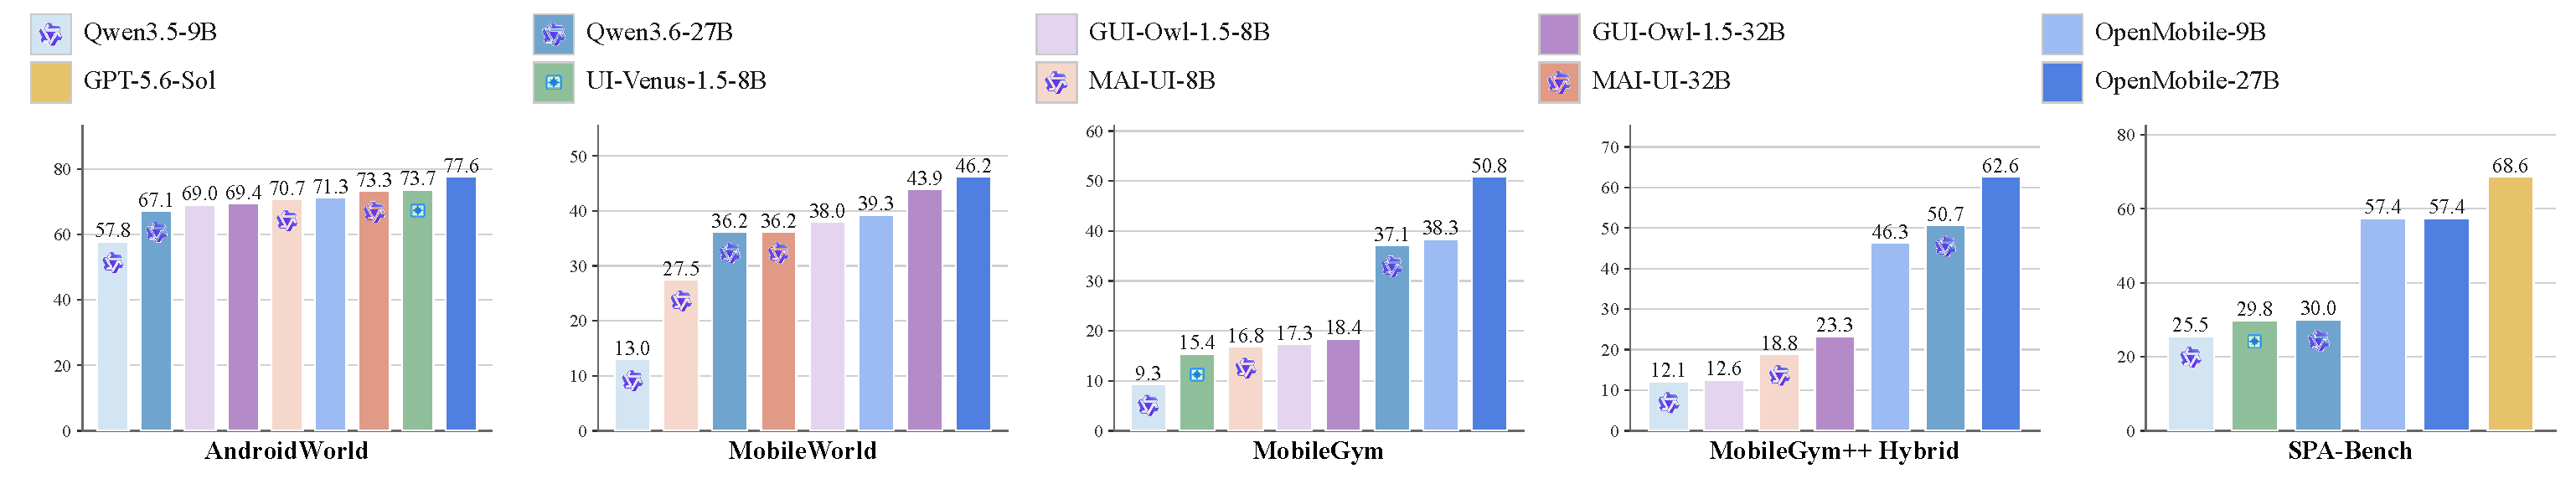
\includegraphics[width=1.0\linewidth]{figures/exp-main-bars.pdf}
    \caption{OpenMobile-2 performs strongly across established mobile agent benchmarks and achieves leading results among open-source models on real-device evaluation.}
    \label{fig:intro-overview}
\end{figure}


% \begin{figure}[h]
% \begin{center}
% \begin{minipage}[b]{0.64\linewidth}
% \centering
% 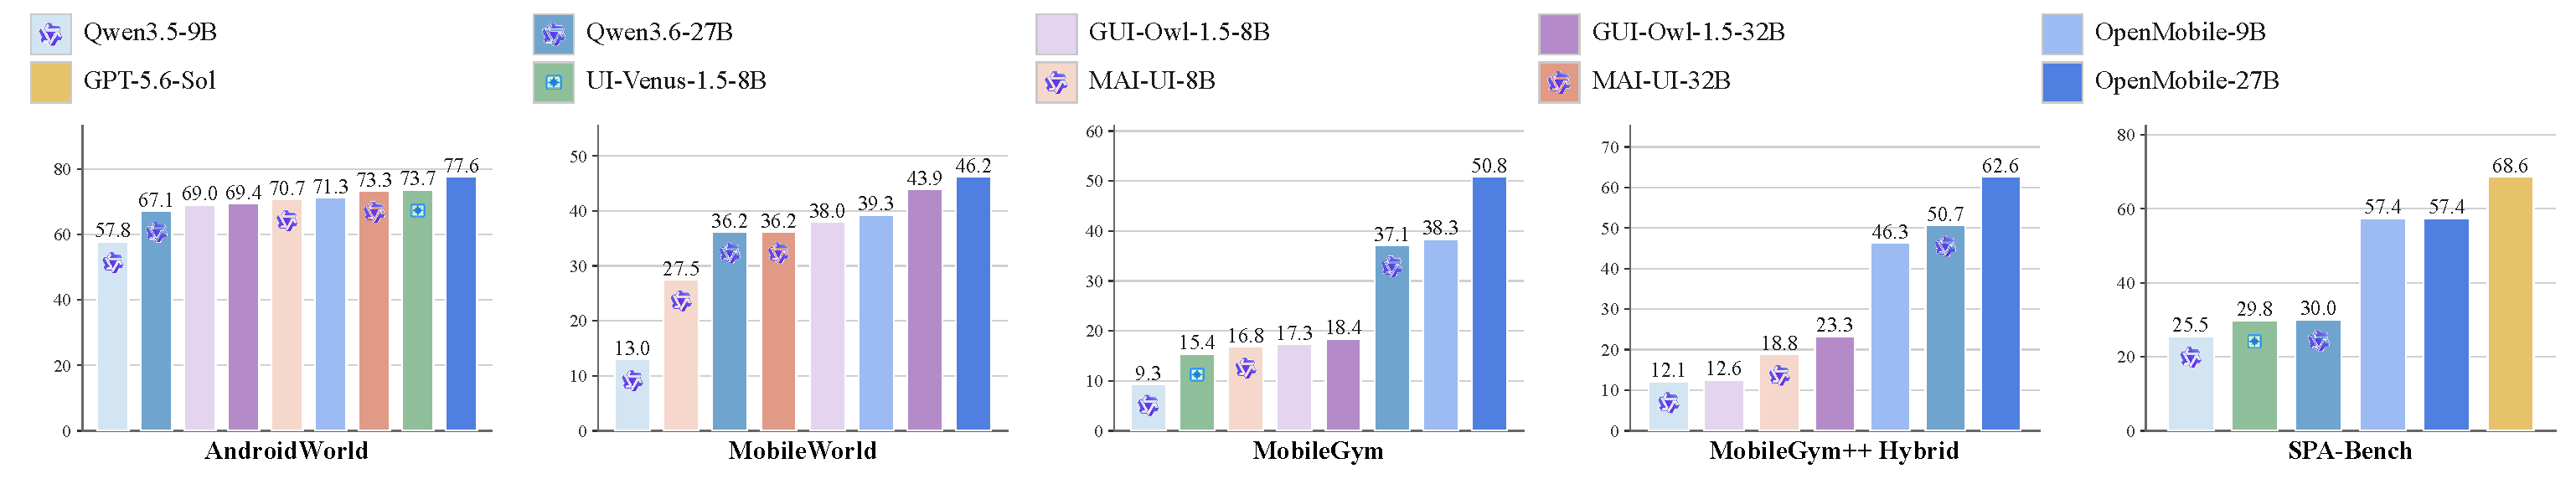
\includegraphics[width=\linewidth]{figures/exp-main-bars.pdf}\\[0.3em]
% {\small (a) AndroidWorld, MobileWorld, MobileGym, and MobileGym++}
% \end{minipage}
% \hfill
% \begin{minipage}[b]{0.25\linewidth}
% \centering
% \includegraphics[width=\linewidth]{figures/exp-spabench-placeholder.pdf}\\[0.3em]
% {\small (b) SPA-Bench}
% \end{minipage}
% \end{center}
% \caption{(a)~Results on established playground and emulator suites.
% (b)~Transfer to real-device SPA-Bench (placeholder).}
% \label{fig:intro-overview}
% \end{figure}


\begin{figure}[t]
\begin{center}
\sbox{\fighybridbox}{\includegraphics[width=0.39\linewidth]{figures/exp-app-pies-9.pdf}}
\begin{minipage}[b]{0.39\linewidth}
\centering
\usebox{\fighybridbox}\\[0.3em]
{\small (a) Application coverage}
\end{minipage}
\hfill
\begin{minipage}[b]{0.59\linewidth}
\centering
\includegraphics[height=\ht\fighybridbox]{{figures/fig2(b)}.pdf}\\[0.3em]
{\small (b) GUI-only vs.\ Hybrid GUI and app-native tools}
\end{minipage}
\end{center}
\caption{(a)~Application coverage of OpenMobile-2. Each square represents two applications; dark and light tiles denote simulator and emulator apps, and dots mark apps with native tools.
(b)~Hybrid GUI and app-native tool use. The same task can be completed through GUI-only interaction (top) or by interleaving GUI actions with app-native tool calls (bottom) over a shared app state.}
\label{fig:intro-hybrid}
\end{figure}

% \begin{figure}[t]
% \centering
% \includegraphics[width=\linewidth]{figures/exp-app-pies-and-tooluse.pdf}
% \caption{(a)~Application coverage in OpenMobile-V2. Each sector is a functional domain; the two bars are mock (dark) and emulator (light) apps.
% (b)~The same in-app task with GUI-only actions (top) versus app-native tools interleaved with GUI actions (bottom).}
% \label{fig:mgpp-app-scale}
% \end{figure}

% Owner: first author
% Scope: OpenMobile-2 --- open agent, diverse environments, training data, hybrid GUI--tool use

\section{Introduction}
\label{sec:intro}

% Such trajectories are costly to collect, and more so on commercial applications, which sit behind login walls and anti-bot checks.

% \sqsc{Mobile agents are evolving toward increasingly capable and general-purpose systems that must operate across diverse applications and workflows. Scaling high-quality interaction data is therefore a promising path toward improving their capabilities and generalization. However, existing approaches to collecting mobile interaction trajectories face inherent scalability challenges. Human demonstrations are costly to collect and annotate, while trajectories gathered directly from real devices require substantial resources to execute, reset, and verify, making it difficult to efficiently scale experience across a broad range of tasks and applications.}
% {Computer-using agents (CUAs) built on vision-language models navigate the digital world as humans do, perceiving and acting through the graphical user interface (GUI). Their progress rests on large volumes of CUA trajectories, task instructions paired with the screens and actions of their execution. 
% Such trajectories are costly to collect,
% and more so on commercial applications, which sit behind login and anti-bot walls.
% Mobile agents in particular are beginning to handle many of a user's daily tasks, yet the leading systems remain opaque in their data, methods, and infrastructure. The open-source community, left with a few public demonstration datasets, fell well behind until trajectory synthesis~\citep{sun2025genesis,cheng2026openmobile} closed much of the gap with proprietary agents on standard benchmarks.}

Mobile agents built on vision-language models are increasingly capable of understanding smartphone interfaces and automating everyday tasks~\citep{wang2025ui, zhou2025mai, xu2026mobile, gao2026ui, zhou2026qwen}.
Such progress depends heavily on large-scale interaction experience, typically in the form of trajectories collected across diverse tasks, applications, and environments~\citep{cheng2026openmobile, team2026ui}. 
Gathering such experience independently is costly, while high-quality interaction data remains largely proprietary, leaving the open community with limited training resources and open models trailing well behind.

% {Computer-using agents (CUAs) built on vision-language models navigate the digital world as humans do, perceiving and acting through the graphical user interface (GUI). 
% Their progress rests on interaction experience (\textit{e.g.}, trajectories) at scale, gathered over many tasks in the environments. 
% Among them, mobile agents are beginning to handle many of a user's daily tasks, 
% yet the leading systems remain opaque in their data, methods, and infrastructure. Gathering such experience independently is costly, and commercial applications add login and anti-bot walls. The open-source community has been left with a few public demonstration datasets and has trailed well behind. Scaling experience efficiently across a broad range of tasks and applications thus remains difficult. \sqs{-> important}}
% reset 部分可以去第三段

% \sqs{Scaling synthesized data further, however, is bounded by the environments that produce it. Synthesized trajectories have so far come from a small set of emulator applications, mostly system utilities and open-source clients, and the distinct tasks each application can host are quickly exhausted.}
% \sqs
% Acquiring such experience at scale without costly human annotation requires a diverse playground of interactive mobile environments for agents to explore. 
% Typical open efforts~\citep{sun2025genesis,cheng2026openmobile} have so far drawn on a small set of emulator applications, 
% mostly open-source apps and system utilities.
% % The distinct tasks each application can host are quickly exhausted.
% % Interaction at scale, 
% Moreover, whether for collecting trajectories or for reinforcement learning, further requires environments that reset cleanly and parallelize cheaply. 
% Existing practices~\citep{rawles2025androidworld,kong2025mobileworld} run real applications inside Android emulators, where third-party applications rarely reset cleanly, and the full Android stack is heavy to replicate at scale. 
% Browser-hosted simulators~\citep{wu2026mobilegym} avoid that overhead, yet their applications remain few and shallow, with no scalable recipe for extending them. 
% Scaling experience therefore requires a diverse playground that holds both kinds of environments, broad in applications, functionally rich, and extendable.

Scaling interaction experience without costly human annotation requires a diverse and controllable mobile playground. 
Especially for commercial applications, reproducing rich workflows and persistent user states at scale has remained a key obstacle.
Existing open efforts~\citep{sun2025genesis,cheng2026openmobile} largely rely on a small set of applications in Android emulators, mostly open-source apps and system utilities. Such environments provide realistic interaction, but third-party apps often lack reliable reset, while the full Android stack is costly to replicate for large-scale rollout and reinforcement learning~\citep{rawles2025androidworld}. Recent simulated environments offer an alternative path~\citep{wu2026mobilegym, liu2026phoneworld}, providing efficient reset and parallelization, yet their applications remain few and shallow, with no scalable recipe for extending them.
% Advancing mobile agent learning therefore calls for a playground spanning broad application domains, with rich functionality and full controllability.

% To overcome the limitations of real-world trajectory collection, recent work has increasingly explored executable mobile environments as a scalable source of training experience. Emulator-based environments enable agents to interact with real applications and generate trajectories through reproducible task execution, but large-scale collection can still be affected by practical constraints of real applications, such as authentication requirements and mutable application states. MobileGym~\citep{wu2026mobilegym} offers a complementary solution by introducing a lightweight and highly controllable mobile simulator, and demonstrates that training experience can be scaled by expanding the underlying application space. However, the simulated applications remain relatively limited in functional richness and interaction depth, constraining the diversity and complexity of experience that can be generated. This motivates the need for a more extensible mobile environment that can support the construction of richer applications and workflows at scale, while retaining the controllability and automatic verification required for large-scale reinforcement learning.

We introduce OpenMobile-2, an open stack of environments, data, and training recipes that puts environment scaling into practice, as shown in Figure~\ref{fig:intro-hybrid}.
% We first build \textsc{MobileGym++}, which substantially expands MobileGym~\citep{wu2026mobilegym} with broader application coverage and greater functional depth. 
We build \textsc{MobileGym++}, a large-scale mobile environment featuring diverse, high-fidelity commercial-style applications, built upon the simulation framework of MobileGym~\citep{wu2026mobilegym}.
In particular, we add 35 functional re-implementations of commercial apps with rich internal state and cross-app workflows, while preserving full controllability for clean reset and verification of task outcomes.
Together with newly configured apps in Android emulator, this forms a diverse training playground spanning over 110 apps. Building on this playground, we curate 12K trajectories for supervised fine-tuning and more than 2K executable tasks for reinforcement learning, each equipped with a reliable verifier.

% We introduce OpenMobile-2, an open stack of environments, data, and training recipes that puts environment scaling into practice, as shown in Figure~\ref{fig:intro-hybrid}.
% % We introduce \textbf{OpenMobile-2}, an open training and evaluation stack that addresses this gap through a controllable yet diverse mobile environment and executable training tasks (Figure~\ref{fig:intro-overview}). 
% % lightweigh simulator
% First,
% % we introduce MobileGym++, a \sqs{lightweight} browser-hosted mobile environment that overcomes the limits of prior emulators by rebuilding commercial applications as mock clients with their own application state.
% We first introduce MobileGym++, a lightweight mobile environment that offers broad coverage of replicated commercial applications and parallelizes cheaply. 
% % We build \textbf{MobileGym++}, adding 35 commercial-style applications and cross-app workflows while preserving clean resets and programmatic verification. 
% % Together with newly configured Android-emulator applications, the playground covers over 110 applications spanning travel, shopping, finance, content, social, office, and local services.
% % Building on this,
% Unlike previous efforts confined to simple utility applications, we newly build 35 functional re-implementations of real commercial applications that derives over 110 playgrounds.
% % we curate over 35 functional re-implementation of real commercial applications with 40 configurations. 
% Each is designed with accessible internal state, so task outcomes are verified directly and workflows can span multiple applications. 
% % Based on our environment,
% % we curate 12K mobile trajectories for supervised fine-tuning and more than 2K executable tasks with automatic rewards for reinforcement learning. 
% Building on this playground, we curate 12K trajectories for supervised fine-tuning and more than 2K executable tasks for reinforcement learning, 
% each equipped with a reliable verifier. 
% We further expose over 300 scoped app-native tools across 50 applications, 
% so that GUI actions and tool calls can be interleaved within the same task. 
% % Beyond the core training setup, we also expose over 300 scoped app-native tools across 50 applications, enabling GUI actions and tool calls to be interleaved within the same task.
% Further, 
% to push mobile-agent evaluation to commercial workflows and hybrid GUI–tool use, 
% we introduce MobileGym++ Bench, 
% a suite of long-horizon tasks on which GUI-only and hybrid policies are fairly compared under the evaluators.
% % This extension allows us to study hybrid GUI--tool interaction in MobileGym++ Bench, where GUI-only and hybrid policies are evaluated on the same long-horizon tasks with the same programmatic checkers.
% % sqs：感觉这里没有体现出面向未来的gui x cli 在 mobile的设计

We further explore an experimental mobile-use setting that combines GUI interaction with app-native tool use. This setting reflects an emerging shift in computer use, where universal but inefficient GUI interaction is increasingly complemented by efficient yet functionally bounded structured interfaces~\citep{hu2026toolcua, shi2026cua}. In \textsc{MobileGym++}, we expose selected app functionalities through over 300 app-native tools across 50 apps, e.g., \textit{search\_course} in a fitness app. This enables us to train agents that interleave GUI actions and tool calls within a task.

% To push mobile agent evaluation toward commercial workflows and hybrid GUI–tool interaction, we introduce \textsc{MobileGym++ Bench}, a suite of 215 long-horizon, cross-app tasks across commercial apps with persistent user states and programmatic verification. It supports both GUI-only and hybrid GUI-tool evaluation on a shared task suite, enabling direct comparison between the two settings.

To push mobile agent evaluation toward real-world commercial workflows and hybrid GUI--tool interaction, we introduce \textsc{MobileGym++ Bench}, a suite of 215 long-horizon cross-app tasks with persistent user states and programmatic verification. Every task can be solved with or without tools, so GUI-only and hybrid agents are compared on the same tasks.
% Performance gained through
% % Agents trained 
% training on our playground and data are shown to transfer across physical devices and emulators in both settings. 
% Experiments show that OpenMobile-2 achieves 77.8 on AndroidWorld, 48.7 on MobileWorld, and 48.4 on MobileGym (Figure~\ref{fig:intro-overview}a),
% % and its gains carry over to real devices. 
% and it further advanced the SPA-Bench performance to 57.4. 
% All environments, data, tools, benchmarks, and training recipes will be open-sourced at XXX.
OpenMobile-2 achieves competitive results on established mobile agent benchmarks, reaching 78.2 on AndroidWorld and 50.4 on MobileWorld.
It further transfers to real-device settings, improving SPA-Bench performance from 25.5 to 57.4 and outperforming substantially larger models.
Further analysis highlights the importance of scaling application diversity for improving agent generalization and reveals the complementary benefits of hybrid GUI and app-native tool use.

% Training with this open stack produces a strong mobile agent that transfers across environments and interaction settings. OpenMobile-2 achieves \textbf{77.8} on AndroidWorld, \textbf{48.7} on MobileWorld, and \textbf{48.4} on MobileGym (Figure~\ref{fig:intro-overview}a), while also transferring to real-device mobile use. These results demonstrate that diverse and verifiable open environments, combined with scalable supervised and executable reinforcement-learning data, can support competitive mobile-agent performance beyond the training playground. More importantly, the unified interface and evaluation framework enables controlled study of GUI-only and hybrid GUI--tool interaction without changing the underlying task or verifier. All environments, data, tools, benchmarks, and training recipes will be open-sourced at XXX.
% beyond infra data contribution，我们还share了recipe and lessons learned on building mobile models
% \sqs{to real device transfer}

Our main contributions are:
\begin{itemize}[leftmargin=2em, itemsep=2pt, topsep=0pt, parsep=0pt]
% \item \textbf{A diverse and verifiable mobile-agent playground.} We introduce MobileGym++, extending a controllable mobile runtime with 35 commercial-style applications and cross-app workflows. Together with newly configured emulator applications, the playground covers over 110 applications while retaining clean resets and programmatic verification.
\item \textbf{Environment Scaling with Replicated Applications.}  MobileGym++ faithfully replicates 35 commercial applications with accessible state in an extendable 110-application playground, overcoming the limited scope of existing open environments.
% controllable 瞰：35 commercial applications 完全可控的感觉
% \item \textbf{Open training data for supervised and reinforcement learning.} We release 12K mobile interaction trajectories and more than 2K executable RL tasks with automatic rewards, together with the corresponding training recipes, enabling scalable training from both demonstrations and environment-grounded feedback.
\item \textbf{Open Training Data and Recipes at Scale.}
We release a fresh collection of 12K diverse trajectories and full recipes, together with 2K+ executable RL tasks with reliable verifiers, which largely advance training mobile agents.
% by reinforcement learning.
\item \textbf{A Unified Framework for GUI and App-native Tool Use.} We integrate over 300 scoped app-native tools across 50 apps and introduce MobileGym++ Bench, where GUI-only and hybrid GUI-tool agents can be trained and evaluated on the same long-horizon tasks. 
% \sqs{todo: squeeze 3 lines each}
\end{itemize}
% Owner: TBD
% Scope: mobile agents (below), mobile environments & data, hybrid GUI--tool use

\section{Related Work}
\label{sec:related}

\paragraph{Mobile Agents.} 
% Mobile agents operate a smartphone from a natural-language instruction, observing the screen and emitting human-like actions such as taps, swipes, and typing until the goal is reached. 
Mobile agents follow natural language instructions to operate smartphones through actions such as taps, swipes, and typing.
% Early systems prompt a proprietary multimodal model behind an external pipeline of screen parsing, planning, and memory~\citep{zhang2025appagent, wang2024mobile}, requiring no training but inheriting the grounding and reasoning limits of that model.
Early systems rely on proprietary multimodal models orchestrated by external pipelines for screen parsing, planning, and memory~\citep{zhang2025appagent, wang2024mobile}, requiring no task specific training.
% Native agents instead pretrain vision-language models for GUI grounding~\citep{cheng2024seeclick, hong2024cogagent, wu2025atlas} and fine-tune them into end-to-end action models~\citep{qin2025ui, liu2024autoglm, ye2025mobile}, which current systems further train with multi-turn reinforcement learning against live devices and sandboxes~\citep{wang2025ui, zhou2025mai, team2026ui, cheng2026openmobile, xu2026mobile, gao2026ui}.
Native agents instead pretrain vision language models for GUI grounding~\citep{cheng2024seeclick, hong2024cogagent, wu2025atlas} and fine-tune them into end-to-end action models~\citep{qin2025ui, liu2024autoglm, ye2025mobile}.
More recent systems further improve these models through multi-turn reinforcement learning on live devices and interactive sandboxes~\citep{wang2025ui, zhou2025mai, team2026ui, xu2026mobile, gao2026ui}.
% This progression makes interaction experience a central resource for scaling mobile agents, spanning high-quality trajectories for supervised training, environments that can reset and parallelize efficiently for reinforcement learning, and executable tasks whose outcomes can be reliably verified and converted into reward.
This progression makes interaction experience a central resource for scaling mobile agents, spanning high-quality trajectories for supervised training, efficiently resettable environments, and verifiable tasks for reinforcement learning.

\paragraph{Trajectory Data and Interactive Environments.}

Existing training trajectories are primarily obtained in two ways. Human-recorded trajectories~\citep{rawles2023androidinthewild, li2024effects, zhang2024android, lu2025guiodyssey} are fixed once collected, expensive to annotate, and carry no executable notion of success. Interactive environments supply the missing loop and differ in how their apps are obtained. One family runs real apps on Android emulators or physical devices and grades tasks against device state~\citep{rawles2025androidworld, xu2025androidlab, chai2026a3, chen2024spa}, which is realistic but resists clean reset and is costly to parallelize; benchmarks over real commercial apps~\citep{wu2026mobilebench, feng2026mobiflow, sui2026androiddaily} inherit these constraints. The other rebuilds apps as controllable mock clients~\citep{trivedi2024appworld, wu2026mobilegym, liu2026phoneworld}, trading fidelity for cheap parallelism, clean reset, and direct state checks. Both are now used as data factories, synthesizing trajectories and verifiable tasks from the environment itself~\citep{sun2025genesis, cheng2026openmobile, liu2026scalewob, cao2026gui, team2026hymobileagent}, making application coverage a key bottleneck for scaling interaction experience.
% Yet controllable apps remain shallow system utilities and open-source clients, leaving commercial workflows only where reset and verification are hardest. 
Yet applications in existing environments remain shallow, with no scalable way to capture interaction experience across commercial workflows.

\paragraph{Hybrid GUI and Tool Use.} 

GUI actions reach any visible control but are slow and brittle; structured calls are efficient but cover only the functions an interface exposes.
% Platforms now surface the latter as App Intents, App Functions, and MCP, and computer-use agents have begun to interleave the two channels~\citep{hu2026toolcua, yan2025mcpworld, jia2026osworld, fan2026screenshots}.
Structured interfaces such as CLIs and MCP are increasingly available alongside GUIs, and recent computer-using agents have begun to combine the two~\citep{hu2026toolcua, yan2025mcpworld, jia2026osworld, fan2026screenshots}.
On mobile the same split appears as API-only worlds with no phone GUI~\citep{trivedi2024appworld}, as external MCP servers attached to a GUI agent~\citep{kong2026mobileworld}, as shortcuts such as RPA over real apps~\citep{zhao2026mas}, or as actions an agent generates from its own GUI traces~\citep{lee2026improving}.
% and as tools synthesized from application state~\citep{lee2026improving}. 
% These settings show that a second channel helps, yet the tools either replace the GUI, sit outside the application, or attach to real apps whose business state is hard to reset and check. What is missing is a mobile environment in which app-native functions and GUI actions write the same store, so GUI-only and hybrid policies can be trained and compared on the same tasks with the same verifier. MobileGym++ supplies that setting.
% In none of these settings do the tools and the GUI act on the same resettable application state, so GUI-only and hybrid agents cannot be trained and compared on the same task under the same verifier. MobileGym++ closes this gap by exposing app-native tools on the same application state as the GUI.
% None of these settings opens its own functions to the agent, and none lets tool calls and GUI actions interleave within one task on the same application state. MobileGym++ simulates this with app-native tools, functions exposed by each replicated application alongside its GUI, so different policies can be trained and compared on the same tasks under the same verifier.
Prior hybrid approaches typically attach external tools or system-level interfaces to a GUI agent, rather than functions exposed by the app itself. In contrast, MobileGym++ simulates commercial apps that selectively expose their own app-native tools alongside the GUI, enabling tool calls and GUI actions to interleave within a task over shared application state.

% TODO: \subsection{GUI and Tool Use}
\section{\textsc{MobileGym++} Playground}
\label{sec:mobilegym++}
\label{sec:method}

\subsection{A gap in controllable commercial applications}
\label{sec:mgpp-env}

Mobile agents are increasingly moving toward real-world workflows across commercial applications, such as travel booking on Trip and online shopping on Taobao, where tasks are often long-horizon and grounded in real user needs. However, training and evaluation environments for such commercial applications remain largely missing, leaving agents with limited opportunities to practice and be evaluated in realistic mobile-use scenarios.

Real-device or Android-emulator setups introduce login friction, irreversible side effects, and costly reset procedures that make large-scale training impractical~\citep{rawles2025androidworld,kong2026mobileworld}. Prior simulated-app work, meanwhile, covers only a narrow range of commercial domains~\citep{wu2026mobilegym,trivedi2024appworld}.

We built MobileGym++, a browser-hosted mobile environment that hosts realistic commercial workflows in controllable simulated applications. The runtime extends MobileGym~\citep{wu2026mobilegym}, preserving its advantages in reset and programmatic evaluation while substantially expanding domain coverage, the number and richness of applications, and support for realistic cross-app workflows. Observations consist of raw screen pixels; there is no accessibility tree and the agent cannot read business state directly. Device state is fully serializable, enabling deterministic reset and parallel instantiation. We newly built 35 commercial applications in this round, bringing the total to 63 installable clients spanning travel, shopping, finance, content, social, office, and local services. Each application maintains persistent business state---orders, budgets, itineraries---that evolves through interaction and supports programmatic task verification.

% Figure~\ref{fig:mgpp-overview} was split out of this section; the overview
% panel now lives in the introduction. Keep the float commented until a
% replacement is dropped into figures/.

% \begin{table*}[t]
% \caption{Comparison of mobile-agent benchmarks on scale, interaction, and evaluation. MobileGym++ uses a 63-application simulated environment of commercial-style apps. The Platform column distinguishes API, Android, and simulated settings. Following recent benchmark comparisons, capabilities are shown as explicit columns. $\checkmark$ denotes supported, $\times$ unsupported, and --- not reported or not applicable. The two MobileGym rows share the same reproducible simulation and deterministic state-based evaluation; scores are omitted because the platforms and task definitions do not share a protocol.}
% \label{tab:mgpp-stack-compare}
% \centering
% \scriptsize
% \setlength{\tabcolsep}{3.0pt}
% \renewcommand{\arraystretch}{1.16}
% \resizebox{\linewidth}{!}{%
% \begin{tabular}{@{}l l r r c c c c c@{}}
% \toprule
%  & & \multicolumn{2}{c}{Scale} & \multicolumn{3}{c}{Interaction} & \multicolumn{2}{c}{Evaluation} \\
% \cmidrule(lr){3-4} \cmidrule(lr){5-7} \cmidrule(lr){8-9}
% Benchmark & Platform & \# Apps & \# Tasks & Cross-app & GUI & Native tools / MCP & Reproducible & Deterministic eval. \\
% \midrule
% AppWorld~\citep{trivedi2024appworld} & API & 9 & 750 / 250 sc. & $\checkmark$ & $\times$ & --- & $\checkmark$ & $\checkmark$ \\
% AndroidLab~\citep{xu2025androidlab} & Android & 9 & 138 & --- & $\checkmark$ & --- & --- & $\checkmark$ \\
% AndroidWorld~\citep{rawles2025androidworld} & Android & 20 & 116 tmpl. & $\checkmark$ & $\checkmark$ & --- & $\checkmark$ & $\checkmark$ \\
% SPA-Bench~\citep{chen2024spa} & Android & 66 & 340 & $\checkmark$ & $\checkmark$ & --- & $\checkmark$ & $\times$ \\
% MobileWorld~\citep{kong2026mobileworld} & Android & 20 & 201 & $\checkmark$ & $\checkmark$ & $\checkmark$ & $\checkmark$ & $\checkmark$ \\
% MobileGym-Bench~\citep{wu2026mobilegym} & Sim. & 28 & 416 tmpl. & $\checkmark$ & $\checkmark$ & --- & $\checkmark$ & $\checkmark$ \\
% \textbf{MobileGym++ Bench (ours)} & \textbf{Sim.} & \textbf{63$^\dagger$} & \textbf{215} & \textbf{$\checkmark$} & \textbf{$\checkmark$} & \textbf{$\checkmark$} & \textbf{$\checkmark$} & \textbf{$\checkmark$} \\
% \bottomrule
% \end{tabular}%
% }
% \vspace{2pt}
% \begin{flushleft}
% \footnotesize
% $^\dagger$ The environment contains 63 installable applications. --- means that the cited benchmark does not report the capability in a comparable form. Deterministic evaluation refers to an automatic, reproducible success check, not a model judge.
% \end{flushleft}
% \end{table*}

\begin{table*}[t]
\caption{Comparison of mobile agent environments across scale, interaction, and controllability. \ding{51} denotes supported, \ding{55} unsupported, and $\sim$ indicates limited system level cross-app interaction support in MobileGym. \# Comm. Apps and \# Tasks denote the number of covered commercial apps and benchmark tasks, respectively. MobileGym++ provides diverse, high-fidelity commercial-style applications with full controllability, while introducing an experimental app-native tool interface.}
\label{tab:mgpp-stack-compare}
\centering
\scriptsize
\setlength{\tabcolsep}{3.0pt}
\renewcommand{\arraystretch}{1.16}
\resizebox{\linewidth}{!}{%
\begin{tabular}{@{}l l c c c c c c@{}}
\toprule
\multirow{2}{*}[-0.6ex]{Environment} 
& \multirow{2}{*}[-0.6ex]{Platform}
& \multicolumn{2}{c}{Scale} 
& \multicolumn{3}{c}{Interaction} 
& \multirow{2}{*}[-0.6ex]{\shortstack{Full\\Controllability}} \\
\cmidrule(lr){3-4} 
\cmidrule(lr){5-7}
& & \# Comm. Apps & \# Tasks  
& Cross-app & GUI & App-native Tools 
& \\
\midrule
AppWorld~\citep{trivedi2024appworld} & API & 9 & 750  
& \ding{51} & \ding{55} & \ding{51} & \ding{55} \\

AndroidLab~\citep{xu2025androidlab} & Emulator & 5 & 138  
& \ding{55} & \ding{51} & \ding{55} & \ding{55} \\

AndroidWorld~\citep{rawles2025androidworld} & Emulator & 0 & 116  
& \ding{51} & \ding{51} & \ding{55} & \ding{55} \\

SPA-Bench~\citep{chen2024spa} & Real-device & 58 & 340  
& \ding{51} & \ding{51} & \ding{55} & \ding{55} \\

MobileWorld~\citep{kong2026mobileworld} & Emulator & 4 & 201  
& \ding{51} & \ding{51} & \ding{55} & \ding{55} \\

MobileGym~\citep{wu2026mobilegym} & Simulator & 12 & 416  
& $\sim$ & \ding{51} & \ding{55} & \ding{51} \\

\textbf{MobileGym++ (ours)} & Simulator & \textbf{35} & \textbf{215}  
& \greencheck & \greencheck & \greencheck & \greencheck \\

\bottomrule
\end{tabular}%
}
\vspace{2pt}
\end{table*}

\subsection{35 high-fidelity commercial applications}
\label{sec:mgpp-apps}

The 35 applications are structurally faithful replicas of their real-world counterparts. Construction starts from the source application's data schema and interaction graph, specified before any interface is rendered, so business-state richness and navigation depth are architectural properties of each replica. Human annotators verify each replica against the live device; the implementation is corrected until the specified routes, state changes, and checks pass (Appendix~\ref{app:mgpp-build}).

Across these clients, the median application exposes 37 routes, 165.5 interactive actions, and 87 page transitions, with a median interaction depth of 3 from the home screen. Relative to the 12 prior MobileGym business apps retained in the same environment, the newly built clients reach $1.48\times$ the interactive actions and $1.91\times$ the page transitions (Figure~\ref{fig:mgpp-app-scale}). The tool channel is described in Section~\ref{sec:mgpp-tools}.

\begin{figure}[t]
\centering
\includegraphics[width=\linewidth]{figures/fig_app_richness_act_trans.pdf}
\caption{App-level interaction richness. Each marker is one app, plotted by its interactive actions and declared page transitions; marker area encodes the number of Bench tasks referencing the app. Filled circles are the newly built commercial clients (colored by domain); open circles are 12 prior MobileGym business apps. Crosses mark group medians: the new clients reach $1.48\times$ the actions and $1.91\times$ the transitions of the prior ones.}
\label{fig:mgpp-app-scale}
\end{figure}


\subsection{Realistic cross-application workflows}
\label{sec:mgpp-crossapp}

Single-application benchmarks cannot detect whether an agent can identify a required value from an external source, carry it across an application boundary, and write it into the correct field---a routine real-device workflow that demands both information retrieval and persistence across isolated state stores.

MobileGym++ places commercial applications on a single resettable device whose shared state is fully serializable, so the exact multi-app starting configuration can be restored for every training episode or evaluation run. Each application maintains its own live business objects---orders, expenses, itineraries, contacts---which evolve through on-screen actions. Clipboard, system broadcasts, and inter-app navigation connect the applications, so a workflow can leave one client and write into another's store rather than merely forwarding a message.

\subsection{Hybrid GUI and app-native tool use}
\label{sec:mgpp-tools}

Commercial applications commonly expose structured lookup and write interfaces alongside their graphical screens, reflecting that the corresponding records would otherwise be reached only through deep GUI navigation. Hybrid interaction---mixing on-screen actions with application-level calls---already appears in prior work~\citep{kong2026mobileworld}. We expose app-native tools according to a simple, principled design: each tool covers structured search or structured writes over an application's own business objects, and every tool call updates the same persistent store as the corresponding GUI action. This equivalence is what enables a controlled comparison---the GUI-only and Hybrid settings share identical tasks, initial states, and terminal checks, so any performance difference isolates the contribution of tool access rather than task selection.

52 applications expose such tools in the foreground, occupying the same action slot as a tap, swipe, or text input. GUI-only remains a complete setting: every task in the benchmark can be completed through the graphical interface. Hybrid adds a second execution path over the same tasks, initial states, and terminal checks, without changing what counts as success.

\subsection{\textsc{MobileGym++ Bench}}
\label{sec:mgpp-bench}

MobileGym++ Bench evaluates whether an agent can complete a commercial write inside resettable simulated applications, when the required value must be recovered through deep in-app navigation and, in cross-app tasks, from another application's live state rather than from the instruction. Existing mobile-agent benchmarks already evaluate single-app GUI operations, and several include cross-application workflows~\citep{rawles2025androidworld,kong2026mobileworld}, but those settings typically terminate on device or backend state rather than on the application's own business objects.

\paragraph{Task Design.}
The primary source of difficulty is commercial navigation and information flow. A single-app task requires the agent to locate, filter, and fill fields across a deep page stack before a business object is written. A cross-application task further requires a live value from another application's store to be identified, carried across the application boundary, and written into the correct field. Instructions are phrased as user goals and do not name widgets, tools, or checker fields; the terminal is a write in the application's own business state.

\paragraph{Scale and Composition.}
The benchmark comprises 215 tasks spanning seven business domains: 109 tasks involve a single application, 74 involve two, 27 involve three, and 5 involve four. Tasks are distributed across applications and business objects so that aggregate performance is not dominated by a small subset of clients.

\paragraph{Evaluation Protocol.}
Each task specifies a user goal, a bound initial state, and a programmatic checker over the before/after diff of application business state. The checker does not inspect the trajectory or screenshots and does not rely on a model judge. GUI-only and Hybrid are evaluated on the same tasks, initial states, and checks. The primary metric is success rate.

% Owner: ________
% Scope: how OpenMobile-Data is collected and why the traces are usable.
% Training recipe stays in Section~\ref{sec:exp-setup}.
\section{OpenMobile-Data}
\label{sec:data}

We release \textbf{OpenMobile-Data}: 12K demonstration trajectories and more than 2K executable RL tasks collected across our Android emulator environments and \textsc{MobileGym++}. The 12K demonstrations are task--trace pairs for imitation, including 1.7K trajectories that interleave GUI actions with app-native tool calls. Each RL task specifies a goal, an initial state, and a programmatic reward, and can be rolled out in MobileGym++ in either GUI-only or hybrid mode.
\subsection{Construction Pipeline}
\label{sec:data-pipeline}
\label{sec:data-collect}

\paragraph{Environment abstraction and task construction.}
To generate executable user goals, the task generator must first know what functionality the environment provides and which operations are available from each state. We therefore explore each application to construct a state--action transition graph, where nodes represent representative application states and edges capture actions that induce state transitions. On the Android emulator, we explore the application to discover screens, actions, and transitions, and consolidate perceptually similar screenshots into representative states. This exploration yields a connected view of the application's functionality: the \textbf{global} view captures the overall state--action structure and available functionality, while the \textbf{local} view captures the actions and states reachable from a particular state. For \textsc{MobileGym++}, the same views are derived directly from the backend specification, which explicitly defines pages, actions, and business objects. Conditioned on these views, Gemini-3.1-Pro-Preview generates realistic and executable user instructions. We filter the generated instructions for quality and diversity, removing low-quality and highly similar tasks.

\paragraph{Trajectory collection and filtering.}
Conditioned on the generated user instructions, Gemini-3.1-Pro-Preview acts as the teacher agent and executes each task in its corresponding environment. The execution follows the available state--action transitions and produces a trajectory of screens, GUI actions, and, where available, native tool calls. We retain only rollouts that complete the specified task and pass the corresponding runtime-specific verifier: completion is assessed by a vision-language judge on the Android emulator, while \textsc{MobileGym++} uses its programmatic task verifier. After collecting successful trajectories, we perform step-level filtering to remove redundant interactions, including meaningless action loops and actions that leave the application state unchanged. The resulting data are released as two separate resources: demonstration trajectories retain the full observation--action sequence, while executable RL tasks retain only the instruction, initial state, and verifier. Details of the verification and filtering procedures are provided in Appendix~\ref{app}.


\subsection{Data Statistics}
\label{sec:data-quality}
\label{sec:data-stats}

\begin{figure}[H]
\centering
\includegraphics[width=\linewidth]{figures/data-quality-3panel.pdf}
\caption{Diversity and coverage of OpenMobile-Data.
\textbf{(a)}~Lorenz curves across seven domains, with Gini coefficients in the legend.
\textbf{(b)}~Pairwise cosine similarity among task goals.
\textbf{(c)}~Fraction of trajectories spanning multiple applications.}

\label{fig:data-quality}
\end{figure}

We characterize OpenMobile-Data from three complementary perspectives: application-domain coverage, task-level similarity, and workflow scope. The data show broad coverage across seven domains, moderate pairwise task similarity (mean cosine similarity 0.43), and substantial cross-app workflows, with 30\% of trajectories spanning multiple applications (40\% on the emulator) (Figure~\ref{fig:data-quality}). Together, these statistics indicate diverse tasks and interaction workflows without strong concentration in any single domain or template.



% Owner: ________
% Scope: setup, baselines, main results, analysis
% Tables and figures for this section live in figures/ with labels prefixed by exp-.
\section{Experiments}
\label{sec:exp}

In this section, we evaluate models trained with OpenMobile-Data on established mobile-agent benchmarks, real-device tasks, and \textsc{MobileGym++}. We use a two-stage curriculum for supervised fine-tuning (SFT): 3 epochs of GUI-only SFT followed by 2 epochs of hybrid SFT on the 11.6K demonstration trajectories. The resulting policy is further trained with RL on 512 tasks randomly sampled from the 2K+ executable tasks. Detailed training configurations are provided in Appendix~\ref{app:details}.


\subsection{Evaluation Benchmarks}
\label{sec:exp-bench}
We evaluate on five benchmarks spanning three evaluation settings---real apps on emulators, simulated commercial apps, and physical devices---as well as GUI-only and tool-augmented interaction. This provides coverage across diverse environments and action spaces. Details are provided in Appendix~\ref{app:eval-bench}.

\textbf{AndroidWorld}~\citep{rawles2025androidworld} contains 116 tasks across 20 real apps on the emulator, with success determined by the resulting device state.

\textbf{MobileWorld}~\citep{kong2026mobileworld} contains 201 harder long-horizon and cross-app tasks, evaluated in both GUI-only and MCP-enabled settings.

\textbf{MobileGym}~\citep{wu2026mobilegym} uses resettable mock apps with state-based verification and reports success rate (SR) and progress rate (PR).

\textbf{\textsc{MobileGym++} Bench} (Section~\ref{sec:mgpp-bench}) contains 215 single- and cross-app tasks evaluated with identical tasks and checkers in GUI-only and hybrid settings.

\textbf{SpaBench}~\citep{chen2024spa} evaluates tasks on physical Android devices, providing a real-device evaluation beyond the emulator-based training environments.

\subsection{Main results}
\label{sec:exp-main}

\begin{table*}[h]
\centering
\caption{\textbf{Main results} on established mobile-agent benchmarks, real-device evaluation, and MobileGym++.
We progressively train each base model with GUI-only SFT, hybrid GUI--tool SFT, and verifiable RL.
Each stage is initialized from the preceding stage.
$*$ denotes results reproduced by us, and
$\pm$ denotes the standard deviation across evaluation seeds.}
\label{tab:main}
\small
\resizebox{\textwidth}{!}{
\begin{tabular}{lccccccccc}
\toprule
Method &
\multicolumn{2}{c}{AndroidWorld} &
\multicolumn{2}{c}{MobileWorld} &
\multicolumn{2}{c}{MobileGym} &
SPA-Bench &
\multicolumn{2}{c}{MobileGym++} \\
\cmidrule(lr){2-3}
\cmidrule(lr){4-5}
\cmidrule(lr){6-7}
\cmidrule(lr){9-10}
&
Pass@1$\uparrow$ & Pass@3$\uparrow$
& GUI & MCP
& SR & PR
& L3
& GUI & MCP \\
\midrule
\multicolumn{10}{c}{\textit{Commercial Models}} \\
\midrule
GPT-5.6-Sol
  & -- & --
  & 70.1 & --
  & -- & --
  & 68.6*
  & -- & -- \\
Gemini-3.1-pro
  & -- & --
  & -- & --
  & -- & --
  & --
  & -- & -- \\
\midrule
\multicolumn{10}{c}{\textit{Open-Weight Models}} \\
\midrule
OpenMobile1-8B
  & 64.7 $\pm$ 3.2 & 78.0
  & 17.7 & --
  & -- & --
  & --
  & -- & -- \\
UI-Venus-1.5-8B
  & 73.7 & --
  & -- & --
  & 15.4 & 28.3
  & 29.8*
  & 19.5* & 16.4* \\
GUI-Owl-1.5-8B
  & 69.0 & --
  & 38.0 & 37.5
  & 17.3* & 31.3*
  & --
  & 13.0* & 12.6* \\
GUI-Owl-1.5-32B
  & 69.4 & --
  & 43.9 & 42.5
  & 18.4* & 30.9*
  & --
  & 18.6* & 23.3* \\
MAI-UI-8B
  & 70.7 & --
  & 27.5 & 20.0
  & 16.8* & 28.3*
  & --
  & 19.2* & 18.8* \\ 
MAI-UI-32B
  & 73.3 & --
  & 36.2 & 30.0
  & -- & --
  & --
  & -- & -- \\
% MAI-UI-235B-A22B
%   & 76.7 & --
%   & 39.7 & 37.5
%   & -- & --
%   & --
%   & -- & -- \\
\midrule
\multicolumn{10}{c}{\textit{OpenMobile-2 (Open-Data Models)}} \\
\midrule
\multicolumn{10}{l}{\textit{9B Model}} \\[-2pt]
Base (Qwen3.5-9B)
  & 57.8 & --
  & 13.0* & 12.5*
  & 9.3* & 20.0*
  & 25.5*
  & 8.0* & 12.1* \\
\quad + GUI SFT
  & 70.0 $\pm$ 2.6 & 81.0
  & 38.5 & 12.5
  & 34.8 & 51.6
  & --
  & 41.1 & 41.9 \\
\quad + Hybrid SFT
  & 69.5 $\pm$ 2.1 & --
  & 39.3 & 27.5
  & 35.9 & 52.2
  & 57.4
  & 39.1 & 44.7 \\
\quad + RL
  & 71.3 $\pm$ 2.4 & 81.0
  & -- & 27.5
  & 38.3 & 52.0
  & --
  & 40.5 & 46.3 \\
\addlinespace
\multicolumn{10}{l}{\textit{27B Model}} \\[-2pt]
Base (Qwen3.6-27B)
  & 67.1 $\pm$ 4.1 *& 81.9*
  & 36.2* & 32.5*
  & 37.1* & 50.1*
  & 30.0*
  & 46.3* & 50.7* \\
\quad + GUI SFT
  & 78.7 $\pm$ 2.1 & 88.8
  & 50.4 & 35.0
  & 44.7 & 58.0
  & --
  & 54.9 & 57.7 \\
\quad + Hybrid SFT
  & 78.2 $\pm$ 3.5 & 87.9
  & 48.7 & 45.0
  & 48.4 & 64.5
  & 57.4
  & 55.3 & 65.6 \\
\quad + RL
  & 77.6 $\pm$ 3.0 & 87.1
  & 46.2 & --
  & 50.8 & 65.1
  & --
  & 55.3 & 62.6 \\
\bottomrule
\end{tabular}
}
\end{table*}

% \paragraph{OpenMobile-Data substantially improves mobile-agent performance.}
% As shown in Table~\ref{tab:main}, models fine-tuned on OpenMobile-Data consistently outperform their corresponding base models across AndroidWorld, MobileWorld, and MobileGym++. The gains are substantial across both model scales, with the 9B model improving by 12.2 points on AndroidWorld and the 27B model by 11.6 points, while the improvements also carry over to MobileWorld and MobileGym++. Beyond the environments used for data synthesis, the resulting models further transfer to real-device interaction: on real Android devices, the full SFT curriculum reaches 57.4 on SPA-Bench L3 for both model scales, substantially above their respective baselines. These results demonstrate that OpenMobile-Data provides broadly transferable interaction experience, highlighting the potential of open trajectory synthesis for building competitive mobile agents.

% \paragraph{Hybrid SFT teaches app-native tool use and generalizes to unseen tools.}
% We train with app-native tools defined by MobileGym++, where each application exposes its own tools and the agent can interleave tool calls with GUI actions while operating on the same underlying app state. As shown above, hybrid SFT substantially increases the benefit of the tool channel on MobileGym++, indicating that the model learns when and how to switch from direct manipulation to higher-level app-native operations. Importantly, this capability is not confined to the tools seen during training. On the MobileWorld MCP evaluation, which involves tools that are not part of the MobileGym++ training environment, hybrid SFT also yields clear gains over GUI-only SFT. This cross-environment improvement suggests that training on app-native tool interactions teaches a more general tool-use behavior: rather than memorizing specific tool APIs, the model learns to recognize when external capabilities are available and incorporate tool calls into its interaction strategy.

\paragraph{OpenMobile-Data improves performance across established mobile-agent benchmarks.}
As shown in Table~\ref{tab:main}, models fine-tuned on OpenMobile-Data consistently outperform their corresponding base models across AndroidWorld, MobileWorld, and MobileGym++. The improvements are substantial at both model scales: the 9B model gains 12.2 points on AndroidWorld, while the 27B model gains 11.6 points, with consistent improvements on MobileWorld and MobileGym++ as well. These results show that the interaction experience synthesized by OpenMobile-Data is useful across different mobile environments.

\paragraph{Performance also transfers to physical devices.}
Beyond established online benchmarks, we evaluate the resulting agents on real Android devices using SPA-Bench L3. The full SFT curriculum reaches 57.4 for both the 9B and 27B models, substantially outperforming their respective base models. This transfer to physical devices provides evidence that the benefits of OpenMobile-Data extend beyond the controlled environments used for training and evaluation, supporting its utility as a source of general mobile interaction experience.

\paragraph{App-native tools improve performance on MobileGym++.}
MobileGym++ enables agents to interleave GUI actions with application-specific tool calls while operating on the same underlying app state. On its benchmark, models trained with hybrid GUI--tool trajectories substantially outperform their GUI-only counterparts, with consistent gains at both model scales (Table~\ref{tab:main}). This result demonstrates that app-native tools provide a useful complementary action channel for mobile interaction.


\paragraph{Hybrid SFT transfers tool-use behavior beyond the training tools.}
We further compare hybrid GUI--tool SFT with GUI-only SFT to examine whether training with app-native tools leads to transferable tool-use behavior. On MobileGym++, hybrid SFT consistently outperforms GUI-only SFT under the same training setup. More importantly, the improvement carries over to MobileWorld MCP, whose tools are not present in the MobileGym++ training environment. This cross-environment transfer suggests that hybrid SFT can teach models to incorporate programmatic capabilities into their interaction strategy beyond memorizing the specific tool APIs observed during training.



% \paragraph{Consistent improvements across established benchmarks.} Training on trajectories collected from our playground leads to substantial improvements over the corresponding base models. On AndroidWorld, Ours-9B improves Pass@1 from 57.3\% to 71.3\%, while Ours-27B reaches 78.2\% Pass@1 and 87.9\% Pass@3. On MobileWorld, Ours-27B achieves 41.9\% GUI success rate, compared with 25.0\% for Qwen3.6-27B. Similarly, on MobileGym, Ours-27B obtains 48.4\% SR and 64.5\% PR, improving over the corresponding baseline by 11.3 and 14.4 percentage points, respectively. These gains across benchmarks with different applications and task distributions indicate that the collected training data transfers beyond the specific applications used during training.

% \paragraph{Hybrid interaction improves task completion.}
% Hybrid GUI--tool interaction provides an effective action space for mobile task completion. On MobileGym++, Qwen3.6-27B improves only marginally from 40.0\% success with GUI-only interaction to 44.4\% with MCP interaction, whereas Ours-27B improves from 48.4\% to 58.1\%. Thus, the trained policy obtains a substantially larger gain from access to native tools, while also outperforming the corresponding base model by 8.4 and 13.7 percentage points in the GUI and MCP settings, respectively. This result demonstrates that the benefits of application-native tool interactions become more pronounced after training on our diverse GUI--tool trajectories.



\label{sec:exp-gui}


\subsection{Analysis}
\label{sec:analysis}

We focus our analysis on two aspects of mobile-agent interaction: how environment coverage relates to transfer, and how app-native tools contribute to task completion.



\begin{figure*}[h]
\centering
\begin{minipage}[t]{0.39\textwidth}
\centering
\vspace{0pt}
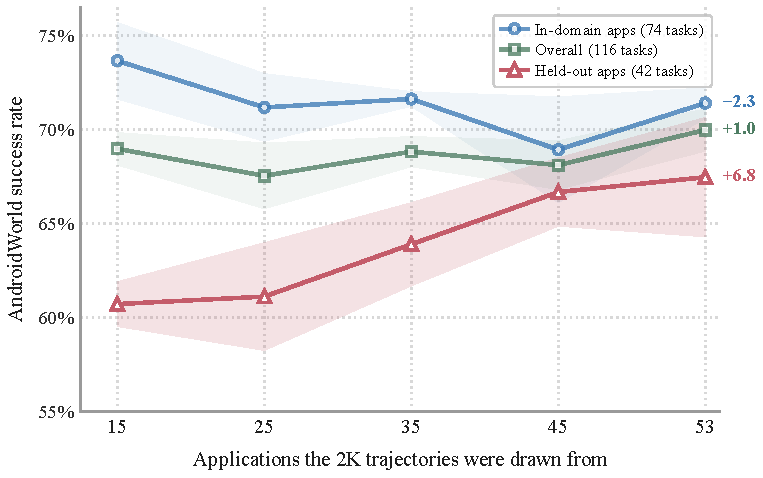
\includegraphics[width=\linewidth]{figures/exp-env-scaling.pdf}\\[-0.2em]
{\small (a) Environment coverage}
\end{minipage}
\hfill
\begin{minipage}[t]{0.59\textwidth}
\centering
\vspace{0pt}
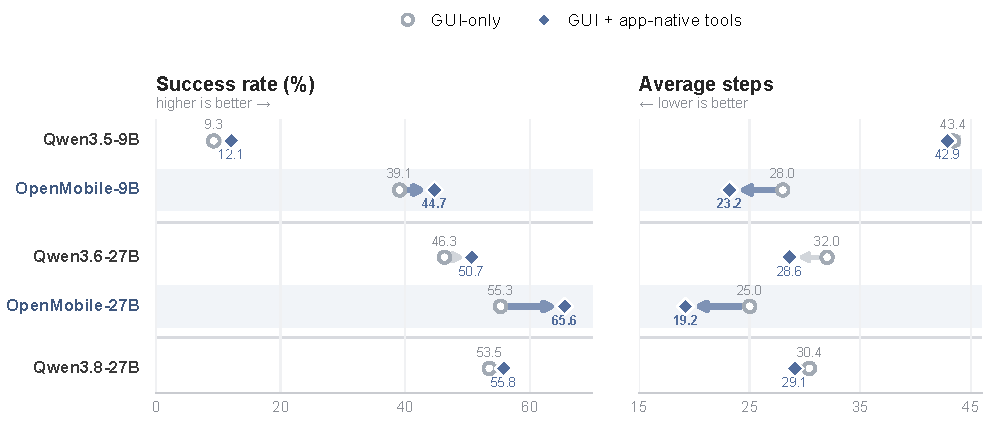
\includegraphics[width=\linewidth]{figures/exp-tool-analysis.pdf}\\[-0.2em]
{\small (b) App-native tool use}
\end{minipage}
\caption{
\textbf{Environment coverage and app-native tool use.}
(a)~Broader coverage improves held-out AndroidWorld performance at a fixed 2K-trajectory budget.
(b)~App-native tools improve success and efficiency, with larger gains after Hybrid SFT.
}
\label{fig:analysis-results}
\end{figure*}


\paragraph{Broader environment coverage improves transfer under a fixed data budget.}
A key question is whether mobile-agent experience benefits more from depth within a few applications or breadth across many applications. We fix the backbone, optimizer, and total training data at 2K emulator trajectories, and vary only the number of applications covered, from 15 to 53; all settings include the same 15 in-distribution (InD) applications. Two observations follow. First, broader coverage improves transfer: Pass@1 on unseen applications rises from 60.7 to 67.5 as coverage grows (Figure~\ref{fig:analysis-results}a). Since the data budget is fixed, this gain comes from breadth rather than from more trajectories. Second, InD performance is maintained even as InD data shrinks. Because the budget is shared, every added application takes trajectories away from the InD applications, and their data share falls from 100\% to 39.1\% (Table~\ref{tab:env-split}); yet InD Pass@1 changes only from 73.7 to 71.4. These results suggest that application coverage provides an additional scaling dimension for mobile-agent experience, with broader coverage improving transfer without substantially compromising performance on familiar applications.


\begin{table}[h]
\centering
\small
\begin{minipage}[t]{0.33\linewidth}
\centering
\caption{Environment-coverage settings under a fixed budget of 2K trajectories. InD data share is the fraction of training trajectories collected in the 15 in-distribution applications shared by all settings.}
\label{tab:env-split}
\setlength{\tabcolsep}{3pt}
\begin{tabular}{cc}
\toprule
\# Train apps & InD data share \\
\midrule
15 & 100\% \\
25 & 64.0\% \\
35 & 48.9\% \\
45 & 41.1\% \\
53 & 39.1\% \\
\bottomrule
\end{tabular}
\end{minipage}
\hfill
\begin{minipage}[t]{0.63\linewidth}
\centering
\caption{\textbf{App-native tool use on MobileGym++.}
TR (tool-call rate) is the average number of app-native tool calls per task, while TSR (tool success rate) is the fraction of tool calls that execute successfully. \#Tools is the number of distinct tools invoked across the benchmark, and \#Tasks is the number of tasks (out of 215) in which at least one app-native tool is called.}


\label{tab:tool_use}
\setlength{\tabcolsep}{3pt}
\begin{tabular}{llcccc}
\toprule
Model & Stage & TR & TSR & \#Tools & \#Tasks \\
\midrule
% Qwen3.8-27B & Base & 0.49 & 99\% & \tbd{} & \tbd{} \\
GUI-Owl-1.5-8B &- &0.58&49\%&15&20\\
GUI-Owl-1.5-32B &- &0.51&78\%&51&45\\
\midrule
\multirow{2}{*}{Qwen3.5-9B} & Base & 0.64 & 94\% & 28 & 21 \\
 & + Hybrid SFT & 1.41 & 78\% & 110 & 113 \\
\midrule
\multirow{2}{*}{Qwen3.6-27B} & Base & 1.64 & 86\% & 97 & 102 \\
 & + Hybrid SFT & 2.23 & 81\% & 115 & 128 \\
\bottomrule
\end{tabular}
\end{minipage}
\end{table}




\paragraph{Hybrid GUI--tool interaction shows substantial untapped potential.}

Simply exposing app-native tools already helps models complete mobile tasks, but existing GUI-only models use them conservatively and capture only a fraction of their potential benefit. Without hybrid training, tool calls occur in only 20--102 of the 215 tasks (Table~\ref{tab:tool_use}), and the resulting improvement remains modest: even the strongest GUI-only baseline gains only 2.3 points from tool access, while no model saves more than 3.4 steps (Figure~\ref{fig:analysis-results}b). Hybrid SFT substantially changes how models exploit the expanded action space. Tool calls increase to 113 and 128 tasks and cover 110 and 115 distinct tools. Although this increased tool usage does not immediately translate into uniformly higher success rates, as models can still make tool-use errors such as selecting unfamiliar tools or providing incorrect arguments, the trained models become substantially more effective when they do use tools. The tool-enabled gain rises to 5.6 points for the 9B model and 10.3 points for the 27B model, while trajectories become 4.8 and 5.8 steps shorter, respectively. This gap between tool availability and effective tool utilization suggests that the main bottleneck is not access to the expanded action space, but learning when, which, and how to invoke tools alongside GUI actions. More broadly, these results suggest that hybrid GUI--tool interaction offers substantial untapped potential: improving models' ability to decide when, which, and how to invoke native tools could unlock further gains from the combined action space.
\section{Conclusion}
\label{sec:conclusion}

We presented OpenMobile-2, an open stack of environments, data, and training recipes for mobile agents. \textsc{MobileGym++} adds 35 controllable commercial-style applications with cross-app workflows and, together with newly configured emulator applications, forms a playground spanning more than 110 applications. From this playground, we curate 12K demonstration trajectories and more than 2K executable RL tasks with reliable verifiers, and expose over 300 app-native tools across 50 applications, enabling GUI actions and tool calls to be interleaved on shared application state. \textsc{MobileGym++ Bench} further provides a unified evaluation of GUI-only and hybrid agents on 215 long-horizon tasks. Together, these components provide an open and scalable foundation for training and evaluating mobile agents.


% Required / recommended statements: do not count toward the page limit.

% Owner: corresponding author (collect input from everyone)
% Required. Does not count toward the page limit. At most 1 page.
% Policy: https://www.iclr.cc/Conferences/2027/AIPolicyForAuthors
% Confirm every item below with the team; the submission form must match this text.
\subsection*{AI use statement}

Generative AI is part of the method studied in this paper, and we also used it as a research and writing aid. We list both uses following the ICLR 2027 AI Policy for Authors.

\textbf{Uses with required disclosure.}
We used generative AI to generate synthetic datasets: Gemini-3.1-Pro-Preview proposes task instructions from explored application states and executes them to produce the candidate trajectories in OpenMobile-Data (Section~\ref{sec:data-pipeline}).
We used generative AI to clean datasets: on the Android emulator, a vision-language judge assesses whether each rollout completes its task, and rollouts it rejects are removed. Trajectories collected in \textsc{MobileGym++} are instead verified by programmatic checkers.
We used AI coding assistants to implement methods: the 35 new \textsc{MobileGym++} applications, their app-native tools, the task checkers, and parts of the training, evaluation, and data-collection pipelines. For each application, the authors first specified the data schema and interaction graph, and the assistants implemented the application against this specification (Section~\ref{sec:mgpp-apps}).
We did not use generative AI to develop theoretical models, formulate or prove mathematical claims, propose hypotheses, or design the research methodology and experiments. We also did not use it to translate text, perform qualitative analysis, or interpret results.

\textbf{Uses with recommended disclosure.}
We used AI assistants to edit and debug software code, to write plotting code for figures, to draft and edit parts of the paper for clarity and structure, and to format references.

\textbf{Verification.}
Human annotators verified every \textsc{MobileGym++} application against the corresponding real client on a device. App-native tools were tested by executing each call and checking the resulting change in application state, and task checkers were validated with test cases and manual spot checks. All synthesized trajectories pass completion checks before release, and the authors manually inspected samples of the released data. All experimental numbers come from our own runs, and all citations were checked against the original sources. We have reviewed all AI-assisted work and take responsibility for the final content of this paper, including text, claims, and artifacts produced with the aid of generative AI.

% Owner: ________
% Recommended. Does not count toward the page limit. At most 1 page.
\subsection*{Ethics statement}

\textbf{Simulated applications and data.}
The \textsc{MobileGym++} applications reproduce the interface structure and business logic of real commercial clients for research purposes. They run entirely in a browser sandbox, do not connect to any real back end, and do not bypass login, anti-bot, or other access controls of the original services. All users, orders, balances, and other records in these applications are synthetic, so the released trajectories and tasks contain no real personal information. Application names and logos are shown only to identify the workflows being replicated; the authors are not affiliated with the corresponding companies.

\textbf{Human involvement.}
Human annotators verified the replicated applications against real clients; they were team members or were compensated at standard rates. No personal data were collected from them, and the study involves no other human subjects.

\textbf{Real-device evaluation.}
Experiments on physical devices used test accounts only and did not complete real payments, orders, or other transactions.

\textbf{Potential misuse.}
Agents that operate phones autonomously could be misused, for example to automate spam, fraud, or unauthorized actions in a user's accounts. Our models are trained and evaluated only in sandboxed environments and on tasks phrased as a user's own goals. We recommend that deployed mobile agents require user confirmation before irreversible actions such as payments and account changes.

% Owner: experiments lead
% Recommended. Does not count toward the page limit.
% Point to code, appendix proofs, and data-processing details; do not dump them here.
\subsection*{Reproducibility statement}

We provide an anonymous repository at \tbd{anonymous link} containing the \textsc{MobileGym++} environment with its applications, app-native tools, and task checkers; \textsc{MobileGym++ Bench}; OpenMobile-Data; and the training and evaluation code. 


% \subsubsection*{Author Contributions}
% Optional. Fill in before camera-ready if desired.
% Author One led Section~\ref{sec:intro}.
% Author Two led Section~\ref{sec:method}.
% Author Three led Section~\ref{sec:exp}.

% \subsubsection*{Acknowledgments}
% Use unnumbered third-level headings for acknowledgments. Funding acknowledgements go here, not in author footnotes.

\bibliography{iclr2027_conference}
\bibliographystyle{iclr2027_conference}

\appendix
\newpage
\section{Training and Evaluation Details}
\label{app:details}

\subsection{Supervised fine-tuning}
\label{app:sft}

\paragraph{Two-stage curriculum.}
Supervised fine-tuning proceeds in two stages that share the hyperparameters in Table~\ref{tab:app-hparams} and differ in their training data (Table~\ref{tab:app-sft-data}). Stage~1 trains for 3 epochs on GUI-only trajectories collected in AndroidWorld, MobileGym, and MobileWorld; app-native tools are not used in this stage. Stage~2 initializes from the Stage~1 checkpoint and trains for 2 epochs on the full mixture, adding 1,774 hybrid trajectories from \textsc{MobileGym++}. GUI trajectories use the GUI-only system prompt in both stages, whereas hybrid trajectories use a tool-aware system prompt.

\paragraph{Training samples.}
Each trajectory yields one training sample per step. A sample contains the task instruction, the interaction history up to that step, and a target turn consisting of a \texttt{Thought:} paragraph followed by one tool call. The three most recent screenshots are retained as images; older screenshots are replaced with the text ``This screenshot has been collapsed.'' The full mixture contains 118,582 step-level samples. SFT screenshots are fed at their native $1080\times2400$ resolution, and the model predicts coordinates in a normalized $999\times999$ space.

\paragraph{Action space.}
Stage~1 uses the \texttt{mobile\_use} tool with actions \texttt{click}, \texttt{long\_press}, \texttt{swipe}, \texttt{type}, \texttt{answer}, \texttt{system\_button} (Back, Home, Menu, or Enter), \texttt{wait}, and \texttt{terminate} (success or failure). Stage~2 adds \texttt{open\_app} and 174 app-native tools, including actions such as \texttt{clock\_\_create\_alarm} and \texttt{notes\_\_create\_note}. An application's tool catalog is available only while that application is in the foreground, so the policy chooses between a GUI action and an available app-native action at each step.

\paragraph{Episode length.}
Training launchers impose no step cap. The longest trajectory in the data has 50 steps. Mean lengths are 11.9 steps for AndroidWorld, 10.7 for MobileGym, 8.8 for MobileWorld, and 6.8 for the hybrid trajectories.

\begin{table}[H]
\centering
\small
\caption{Training hyperparameters for the 9B model. SFT values are shared by both stages; -- indicates that a setting does not apply.}
\label{tab:app-hparams}
\setlength{\tabcolsep}{3pt}
\begin{tabular}{p{0.27\linewidth}p{0.32\linewidth}p{0.32\linewidth}}
\toprule
Hyperparameter & SFT & RL \\
\midrule
Framework & Megatron-SWIFT & verl \\
Objective & Next-token prediction & DAPO (group-relative) \\
Trainable parameters & LLM (vision frozen) & LoRA \\
Optimizer & Adam ($\beta_1{=}0.9$, $\beta_2{=}0.95$) & AdamW \\
Weight decay / gradient clip & 0.1 / 1.0 & 0.1 / 1.0 \\
Learning rate & $5\times10^{-6}$ & $1\times10^{-6}$ \\
Schedule & Cosine; 3\% warmup; minimum $10^{-7}$ & 40 warmup steps \\
Batch size & 32 (microbatch 1) & 64 tasks $\times$ 8 rollouts \\
Training length & 3 + 2 epochs & 200 steps; 2 updates each \\
Group size & -- & 8 \\
Clipping $\epsilon_{\text{low}}$ / $\epsilon_{\text{high}}$ & -- & 0.2 / 0.28 \\
KL coefficient & -- & 0.001 (low-variance estimator) \\
Token budget & 32,768 (packed) & 22,528 (1,024 per turn) \\
Screenshot input & $1080\times2400$ (native) & Short side 512 px \\
Screenshot history & Last 3 & Full episode \\
Coordinate space & $999\times999$ & $999\times999$ \\
Step cap & None (maximum observed: 50) & 30 (GUI-only); 25 (hybrid) \\
Precision & bf16 & bf16 \\
Hardware & 8 GPUs; tensor parallelism 4 & 32 H100 GPUs; sequence parallelism 8 \\
\bottomrule
\end{tabular}
\end{table}

\begin{table}[t]
\centering
\small
\caption{Trajectories included in each SFT stage. Steps are step-level training samples.}
\label{tab:app-sft-data}
\setlength{\tabcolsep}{4pt}
\begin{tabular}{p{0.36\linewidth}rrcc}
\toprule
Source & Trajectories & Steps & Stage 1 & Stage 2 \\
\midrule
AndroidWorld environment & 5,026 & 59,806 & Yes & Yes \\
MobileGym & 2,144 & 22,857 & Yes & Yes \\
MobileWorld environment & 2,699 & 23,825 & Yes & Yes \\
\textsc{MobileGym++} hybrid & 1,774 & 12,094 & -- & Yes \\
\midrule
Stage 1 total & 9,869 & 106,488 & Yes & -- \\
Stage 2 total & 11,643 & 118,582 & -- & Yes \\
\bottomrule
\end{tabular}
\end{table}

\subsection{Reinforcement learning}
\label{app:rl}

\paragraph{Algorithm.}
We initialize reinforcement learning from the Stage~2 SFT checkpoint and optimize the policy with GRPO-style group-relative advantages~\citep{shao2024deepseekmath} and the DAPO objective~\citep{yu2026dapo}, implemented in verl~\citep{sheng2025hybridflow}. For each task, we sample a group of 8 rollouts in \textsc{MobileGym++} and use asymmetric clipping with $\epsilon_{\text{low}}{=}0.2$ and $\epsilon_{\text{high}}{=}0.28$. We apply a KL penalty to the SFT reference policy using a low-variance estimator. The hyperparameters are listed in Table~\ref{tab:app-hparams}.

\paragraph{Tasks.}
RL tasks are drawn from the more than 2,000 executable tasks in OpenMobile-Data (Section~\ref{sec:data}). Each task has a bound initial state and a programmatic verifier in \textsc{MobileGym++}. We randomly sample 512 tasks: 448 for training and 64 for validation.

\paragraph{Rollouts.}
Each rollout is a multi-turn episode. Every assistant turn contains a \texttt{Thought:} paragraph and one tool call, with at most 1,024 generated tokens per turn. Unlike SFT, the full screenshot history remains in context. The action space contains nine \texttt{mobile\_use} actions (including \texttt{open\_app}) and, in the hybrid setting, 333 app-native tools. An application's tool catalog is provided when it comes to the foreground; each tool call returns a structured receipt containing its output or an error code. An episode ends when the agent calls \texttt{terminate} or reaches the smaller of the task-specific and global step limits (Table~\ref{tab:app-hparams}).

\paragraph{Reward.}
The reward of a rollout is
\begin{equation*}
r = \underbrace{v}_{\text{verifier}} \cdot \underbrace{p}_{\text{process check}} \cdot \underbrace{m_{\text{tool}}}_{\text{tool bonus}} \cdot \underbrace{\ell}_{\text{length factor}},
\end{equation*}
where $v\in\{0,1\}$ is the programmatic task-verifier outcome and $p\in\{0,1\}$ is an LLM-judge process check. The process check rejects degenerate behavior, including garbled output, repetitive loops, failure to terminate, and protocol violations. In hybrid runs, $m_{\text{tool}}=2$ when the judge finds that a tool call made substantive task progress, and $m_{\text{tool}}=1$ otherwise. The length factor $\ell$ is 1 for responses up to 12,000 tokens and decreases linearly to 0.5 at the response budget.

\paragraph{Infrastructure.}
Training runs on 32 H100 GPUs across 4 nodes. Each node hosts a \textsc{MobileGym++} simulator, and rollouts drive up to 512 browser-hosted devices concurrently. Rollouts are generated with vLLM; the actor is trained with FSDP2 and Ulysses sequence parallelism of degree 8.

\subsection{Evaluation benchmarks}
\label{app:eval-bench}

We evaluate on five benchmarks that differ in where the apps run, which actions the agent may take, and how completion is judged, so a gain that holds on all of them is unlikely to come from fitting one environment.

\textbf{AndroidWorld}~\citep{rawles2025androidworld} is a widely adopted benchmark for evaluating mobile agents in reproducible Android environments. It comprises 116 programmatic tasks across 20 real-world apps, with deterministic evaluation based on the resulting device state. We report task success rate.

\textbf{MobileWorld}~\citep{kong2026mobileworld} is a recent benchmark designed to evaluate more challenging mobile-agent capabilities. It contains 201 tasks across 20 apps, with an emphasis on long-horizon and cross-application workflows. We evaluate both its GUI-only tasks and MCP-enabled tasks using the official task checker.

\textbf{MobileGym}~\citep{wu2026mobilegym} is a benchmark built around resettable mock applications with programmatic state-based evaluation. It evaluates agents on tasks requiring application interactions and state transitions, and reports both success rate (SR) and progress rate (PR), capturing complete and partial task completion, respectively.

\textbf{\textsc{MobileGym++} Bench} (Section~\ref{sec:mgpp-bench}) is designed to evaluate mobile agents on tasks involving application business state and native tool interactions. It contains 215 tasks spanning single-app and cross-app workflows, each initialized from a fixed application state and evaluated by a programmatic checker over the application business state. We evaluate both GUI-only and hybrid GUI--MCP interaction on the same tasks, initial states, and checker.

\textbf{SpaBench}~\citep{chen2024spa} evaluates mobile agents on real Android devices, providing an evaluation setting that goes beyond the controlled emulator and simulator environments used in training and the other benchmarks. We use SpaBench to assess whether the capabilities learned from OpenMobile-2 transfer to real-device interaction.

\section{MobileGym++ App Construction}
\label{app:mgpp-build}

\paragraph{Behavior specification.}
We represent core application workflows as a structured graph of page nodes and meaningful UI states. Each state-changing interaction names its UI element and action, describes the expected state effect, and includes a check for the resulting state. This makes navigation and business-state writes explicit before implementation. The specification is then used as the contract for implementing and checking routes, actions, and state changes.

\par\medskip
\noindent
\begin{minipage}{\linewidth}
\centering
\includegraphics[width=\linewidth]{figures/app-construction-process.pdf}
\captionof{figure}{Illustrative single-app workflow. The phone screens show one journey; the numbered circles mark construction stages, not application counts.}
\label{fig:app-construction-process}
\end{minipage}
\par\medskip

\paragraph{Specification entry.}
The excerpt below shows the form of a state-changing interaction. A page identifier groups its controls; the action identifier names the operation; and the state change and check make the outcome observable.
\begin{minipage}{\linewidth}
\begin{lstlisting}[basicstyle=\ttfamily\small, frame=single, columns=fullflexible, breaklines=true]
{
  "id": "detail.skuPanel",
  "interactions": [{
    "element": "Add to cart",
    "effect": "state",
    "actionId": "sku.addToCart.confirm",
    "stateChange": "cart.items += item",
    "stateCheck": "item and quantity match"
  }]
}
\end{lstlisting}
\end{minipage}

\paragraph{Implementation and checks.}
Routes and actions operate on app-owned state and seeded data. GUI actions and app-native tools use the same app state. A coverage check maps declared interaction identifiers to implementation bindings; runtime replay checks representative transitions and their expected state effects. When a mismatch appears, the specification is corrected and the affected checks are replayed. Each delivered app includes its executable interface, state model, seeded data, and reusable checks for core flows. Benchmark instructions and terminal verifiers are authored separately on top of the completed apps.


\section{Playground Inventory}
\label{app:mgpp-apps}

\textsc{MobileGym++} contains 63 installable simulated clients: 35 applications built in this work and 28 inherited from MobileGym. The 63 clients comprise 49 commercial-style applications and 14 system clients. The Android emulator inventory contains 62 applications. The tables below list applications by domain; the emulator inventory is not divided by source batch.

\begin{table}[H]
\centering
\small
\caption{Application counts by domain in the two runtimes.}
\label{tab:app-domain-counts}
\begin{tabular}{lrr}
\toprule
Domain & \textsc{MobileGym++} & Emulator \\
\midrule
Lifestyle & 18 & 19 \\
Productivity & 15 & 23 \\
Entertainment & 9 & 15 \\
Shopping & 8 & 1 \\
Travel & 5 & 3 \\
Social & 6 & 0 \\
Finance & 2 & 1 \\
\midrule
Total & 63 & 62 \\
\bottomrule
\end{tabular}
\end{table}

\subsection{MobileGym++ applications}
\label{app:mgpp-app-table}

Table~\ref{tab:app-new-tools} lists the 35 applications built in this work by domain and app-native tool count. A zero means that the application exposes no app-native tools. Table~\ref{tab:app-mgpp-list} gives the complete 63-client inventory.

\begin{table}[t]
\centering
\small
\caption{The 35 applications built in this work, with app-native tool counts.}
\label{tab:app-new-tools}
\setlength{\tabcolsep}{5pt}
\begin{tabular}{llr}
\toprule
Domain & Application & Native tools \\
\midrule
Entertainment & Podcasts & 8 \\
Entertainment & Fanqie Novel & 0 \\
Entertainment & Tencent Video & 0 \\
Entertainment & Ximalaya & 0 \\
Entertainment & Youku & 0 \\
Finance & Kapi & 8 \\
Lifestyle & Baicizhan & 0 \\
Lifestyle & Cainiao & 0 \\
Lifestyle & Dianping & 10 \\
Lifestyle & Keep & 0 \\
Lifestyle & Luckin Coffee & 7 \\
Lifestyle & Maoyan & 0 \\
Lifestyle & Meiyou & 0 \\
Lifestyle & Meituan & 0 \\
Productivity & Daily & 0 \\
Productivity & BOSS Zhipin & 0 \\
Productivity & Days Matter & 9 \\
Productivity & TickTick & 8 \\
Productivity & Fanqie ToDo & 0 \\
Productivity & flomo & 0 \\
Productivity & Google Drive & 8 \\
Productivity & Mail & 8 \\
Productivity & Slack & 9 \\
Shopping & JD & 13 \\
Shopping & Pinduoduo & 0 \\
Shopping & Suning & 0 \\
Shopping & Taobao & 14 \\
Shopping & Taobao Instant Commerce & 10 \\
Shopping & Vipshop & 0 \\
Shopping & Xianyu & 0 \\
Social & Douban & 0 \\
Social & Weibo & 0 \\
Travel & Ctrip & 8 \\
Travel & DiDi & 0 \\
Travel & Qunar & 0 \\
\bottomrule
\end{tabular}
\end{table}

\begin{table}[t]
\centering
\small
\caption{The 63 \textsc{MobileGym++} clients. $^\dagger$ marks system clients; all other entries are commercial-style applications.}
\label{tab:app-mgpp-list}
\begin{tabular}{lp{0.74\linewidth}}
\toprule
Domain & Applications \\
\midrule
Lifestyle (18) & Baicizhan, Cainiao, Dianping, Keep, Luckin Coffee, Maoyan, Meituan, Meiyou, Weather, Answer Sheet$^\dagger$, Browser$^\dagger$, Calculator$^\dagger$, Calculator~2$^\dagger$, Clock$^\dagger$, Compass$^\dagger$, Gallery$^\dagger$, Settings$^\dagger$, Themes$^\dagger$ \\
Productivity (15) & BOSS Zhipin, Days Matter, TickTick, Fanqie ToDo, flomo, Google Drive, Mail, Slack, Daily, Tencent Meeting, Calendar$^\dagger$, Phone$^\dagger$, Files$^\dagger$, Notes$^\dagger$, Messages$^\dagger$ \\
Entertainment (9) & Podcasts, Fanqie Novel, Tencent Video, NetEase Cloud Music, Ximalaya, Youku, Bilibili, Spotify, WeRead \\
Shopping (8) & JD, Pinduoduo, Suning, Taobao, Taobao Instant Commerce, Vipshop, Xianyu, eBay \\
Travel (5) & Ctrip, DiDi, Qunar, Maps, Railway 12306 \\
Social (6) & Douban, Weibo, RedNote, Reddit, WeChat, X \\
Finance (2) & Alipay, Kapi \\
\bottomrule
\end{tabular}
\end{table}

\subsection{Emulator applications}
\label{app:emu-apps}

\begin{table}[t]
\centering
\small
\caption{The 62 Android emulator applications, grouped by domain.}
\label{tab:app-emu-list}
\begin{tabular}{lp{0.74\linewidth}}
\toprule
Domain & Applications \\
\midrule
Lifestyle (19) & Camera, Chrome, Clock, Settings, Simple Gallery Pro, AndroidWorld, Broccoli, Clipper, MiniWoB, OpenTracks, APKPure, Breezy Weather, Coursera, DuckDuckGo, F-Droid, NerdCalci, Snapseed, Quark, Xiachufang \\
Productivity (23) & Files, Contacts, Dialer, Simple SMS Messenger, Simple Calendar Pro, Joplin, Markor, Tasks, Simple Draw Pro, Audio Recorder, Amaze, Material Files, MiXplorer, MT Manager, Etar, Omni Notes FOSS, Code Editor, DeepL, GeminiAssist, Doubao, Element, Mattermost, Session \\
Entertainment (15) & VLC, Retro Music, iQIYI, Youku, Bilibili, NetEase Cloud Music, NewPipe, AntennaPod, Toutiao, Yahoo News, Yahoo Sports, Wikipedia, Librera, 2048, Angry Birds Friends \\
Shopping (1) & eBay \\
Travel (3) & OsmAnd, Booking.com, Citymapper \\
Finance (1) & Pro Expense \\
\bottomrule
\end{tabular}
\end{table}

\section{Data Collection}
\label{app:data}

\subsection{Construction details}
\label{app:sft-data}

\paragraph{Environment representation and task synthesis.}
Task synthesis is grounded in the functions an application supports and the states reachable from a given screen. For Android emulator applications, exploration is used to map screens and transitions. For \textsc{MobileGym++}, the page, action, and business-object declarations are available from each simulated client. A global view summarizes an application's features and where they are located; a local view lists states directly reachable from the current screen. Instructions are phrased as user goals rather than naming the controls, tools, or verifier fields to use.

\paragraph{Trajectory rollout and filtering.}
The same model executes each instruction step by step, producing a \texttt{Thought:} paragraph followed by one action per turn. When the foreground application exposes app-native tools, its tool catalog is available and the model may choose a tool call or GUI action. Both channels act on the same application state. A rollout is retained when the task succeeds under its runtime-specific check: the programmatic verifier for \textsc{MobileGym++} or a vision-language judge for Android emulator tasks. Degenerate transitions that leave application state unchanged are removed.

\subsection{Executable RL tasks}
\label{app:rl-data}
Each executable RL task is a triple of instruction, initial state, and verifier. The initial state is a snapshot of the \textsc{MobileGym++} application stores, so repeated rollouts of a task start from the same state. The verifier compares application state before and after an episode and checks whether the requested change was written. Since it reads application state rather than the screen, it evaluates GUI and app-native tool actions alike.

\subsection{Data composition}
\label{app:data-quality}

\paragraph{Source coverage.}
The SFT mixture contains 11,643 trajectories. Of these, 7,725 come from AndroidWorld and MobileWorld (about two thirds), while 3,918 come from MobileGym and \textsc{MobileGym++} (about one third; Table~\ref{tab:app-sft-data}). The mixture therefore combines trajectories from Android emulator applications with controllable simulated-client workflows.

\paragraph{Trajectory length and action channels.}
Mean trajectory lengths range from 6.8 steps for hybrid trajectories to 11.9 for AndroidWorld, with MobileGym at 10.7 and MobileWorld at 8.8. The 1,774 hybrid trajectories use 174 distinct app-native tools; GUI actions remain available alongside these tools.

\section{MobileGym++ Bench}
\label{app:mgpp-bench}

The following subsections document the task split and domain distribution for MobileGym++ Bench, and give two worked examples that illustrate the evaluation protocol concretely.

\subsection{Task composition}
\label{app:mgpp-bench-split}
The 215 tasks span one to four applications. Of these, 109 use one app, 74 use two, 27 use three, and 5 use four; 106 tasks therefore require cross-app interaction. Figure~\ref{fig:bench-composition} and Table~\ref{tab:bench-domain-incidence} report the same split and the task incidences by domain. Because a cross-domain task is counted once in each domain it touches, these incidences overlap and do not sum to 215.

\begin{figure}[t]
\centering
\includegraphics[width=\linewidth]{figures/fig_bench_composition.pdf}
\caption{MobileGym++ Bench composition. Left: tasks by the number of applications they touch. Right: task incidences by domain. Domain counts are not mutually exclusive.}
\label{fig:bench-composition}
\end{figure}

\begin{table}[t]
\centering
\small
\caption{MobileGym++ Bench task incidences by domain. A task that touches more than one domain is counted in each, so the column does not sum to 215.}
\label{tab:bench-domain-incidence}
\begin{tabular}{lr}
\toprule
Domain & Task incidences \\
\midrule
Productivity & 97 \\
Finance & 34 \\
Shopping & 53 \\
Social & 35 \\
Entertainment & 26 \\
Lifestyle & 46 \\
Travel & 29 \\
\bottomrule
\end{tabular}
\end{table}

\subsection{Example tasks}
\label{app:mgpp-bench-ex}

\paragraph{GUI-only: transfer search results into Notes.}
Task 202 (\texttt{HTV6Case27}) asks the agent to search Xiaohongshu using the Chinese term for travel, identify the two most-liked posts among the first ten results, and write their full titles to the system Notes app, one per line (not to flomo). In the GUI-only setting, the agent can use the \texttt{mobile\_use} interface actions but receives no app-native tools. The programmatic checker independently retrieves the top two titles from the initial search results and verifies that both appear in the latest Notes entry.

\paragraph{Hybrid: complete a Taobao purchase.}
Task 111 (\texttt{HTV6Case69}) asks the agent to buy a Jianmu large-capacity insulated flask made of 316 stainless steel, choose the saved address marked School, and pay using Huabei installments. The hybrid action set combines GUI actions with Taobao app-native tools; relevant calls include \texttt{taobao\_\_search\_items}, \texttt{taobao\_\_get\_item\_summary}, and \texttt{taobao\_\_add\_to\_cart}. \texttt{taobao\_\_prepare\_checkout} opens the confirmation page as a non-persisted draft, so the agent must still complete the payment flow in the GUI. The checker requires a new paid order for the target item, with the school-tagged address and Huabei installment payment recorded in the order.

\section{App-native tool examples}
\label{app:tool-schema}
App-native tools occupy the same action slot as \texttt{mobile\_use} GUI interactions: at each step, the agent chooses one action from a single list that includes both. When an application is in the foreground, its tool catalog is appended to that list; when the application leaves the foreground, its tools are removed. The following Taobao schemas illustrate read, state-changing, and navigation-to-GUI operations. The tool handlers and the visible application use the same \texttt{useTaobaoStore}: for example, \texttt{add\_to\_cart} updates the cart state that the GUI renders. Tool schemas reject undeclared input keys.

\begin{lstlisting}[basicstyle=\ttfamily\small,frame=single,breaklines=true]
taobao__search_items(query: string, limit?: integer)
taobao__get_item_summary(item_id: string)
taobao__add_to_cart(item_id: string, sku_description: string,
                    quantity: integer [1..99])
taobao__prepare_checkout(cart_line_ids: string[1..30])
\end{lstlisting}

The first two calls read the catalog; \texttt{add\_to\_cart} validates the item, SKU, and quantity before writing the shared cart. \texttt{prepare\_checkout} accepts one to 30 valid cart-line IDs, opens the confirmation page, and creates neither an order nor a payment. The GUI then continues from the same app state.

\section{System prompt}
\label{app:sys-prompt}
All models are evaluated with the system prompt below. The GUI tool \texttt{mobile\_use} is always available; when an application exposes app-native tools, the environment lists them in the tool message for as long as that application stays in the foreground. In the GUI-only setting no such catalog is attached. The JSON schema is broken across lines for readability.

\promptfile{System prompt for GUI-only and hybrid evaluation}{prompts/system_prompt.txt}


\end{document}
